% Explication des étapes de l'alogorithme par un exemple d'Evaluation:

\section{Algorithm simulation}
\label{algo_but}

In this section we demonstrate how our methode permits to generate a PH model coherent to the set of biological regulatory time series data given as an input. 
First, the method uses discritised observations as an input, thus it is necessary to use an other method which transforms the analogic time series data to discritised time series data.

%\begin{figure}[htb!]
%Observations:\\
%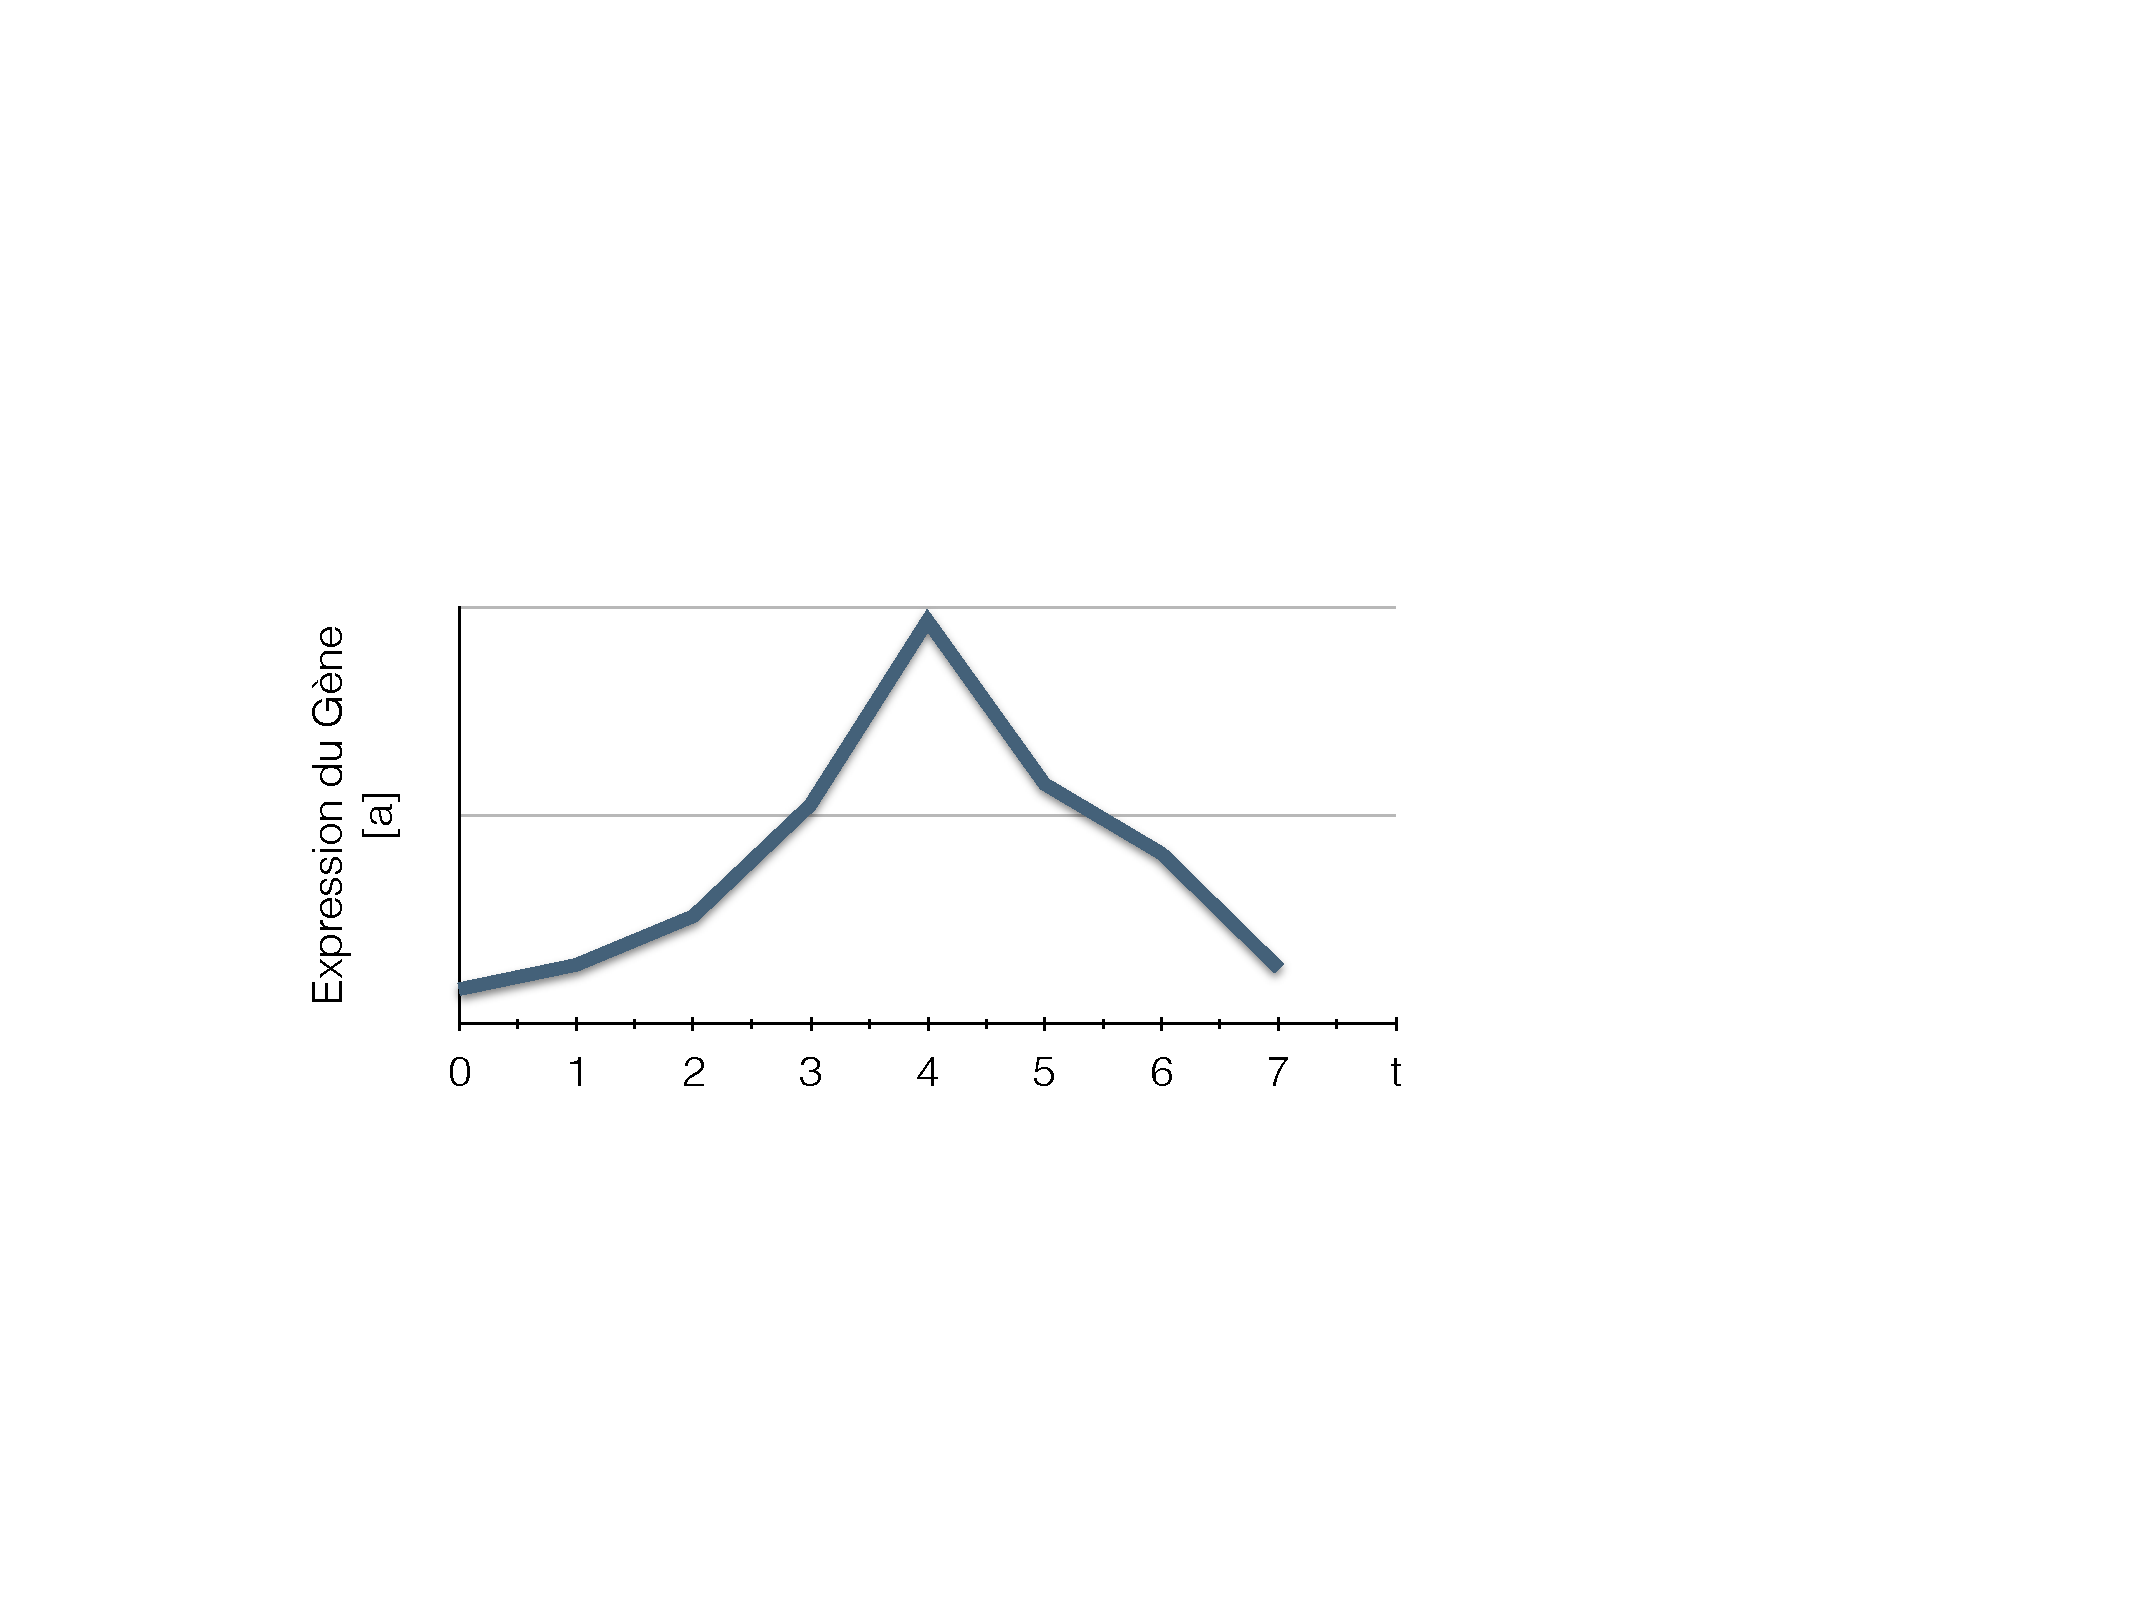
\includegraphics[ width =0.35\linewidth]{images/courbes/gene-a.pdf}\\
%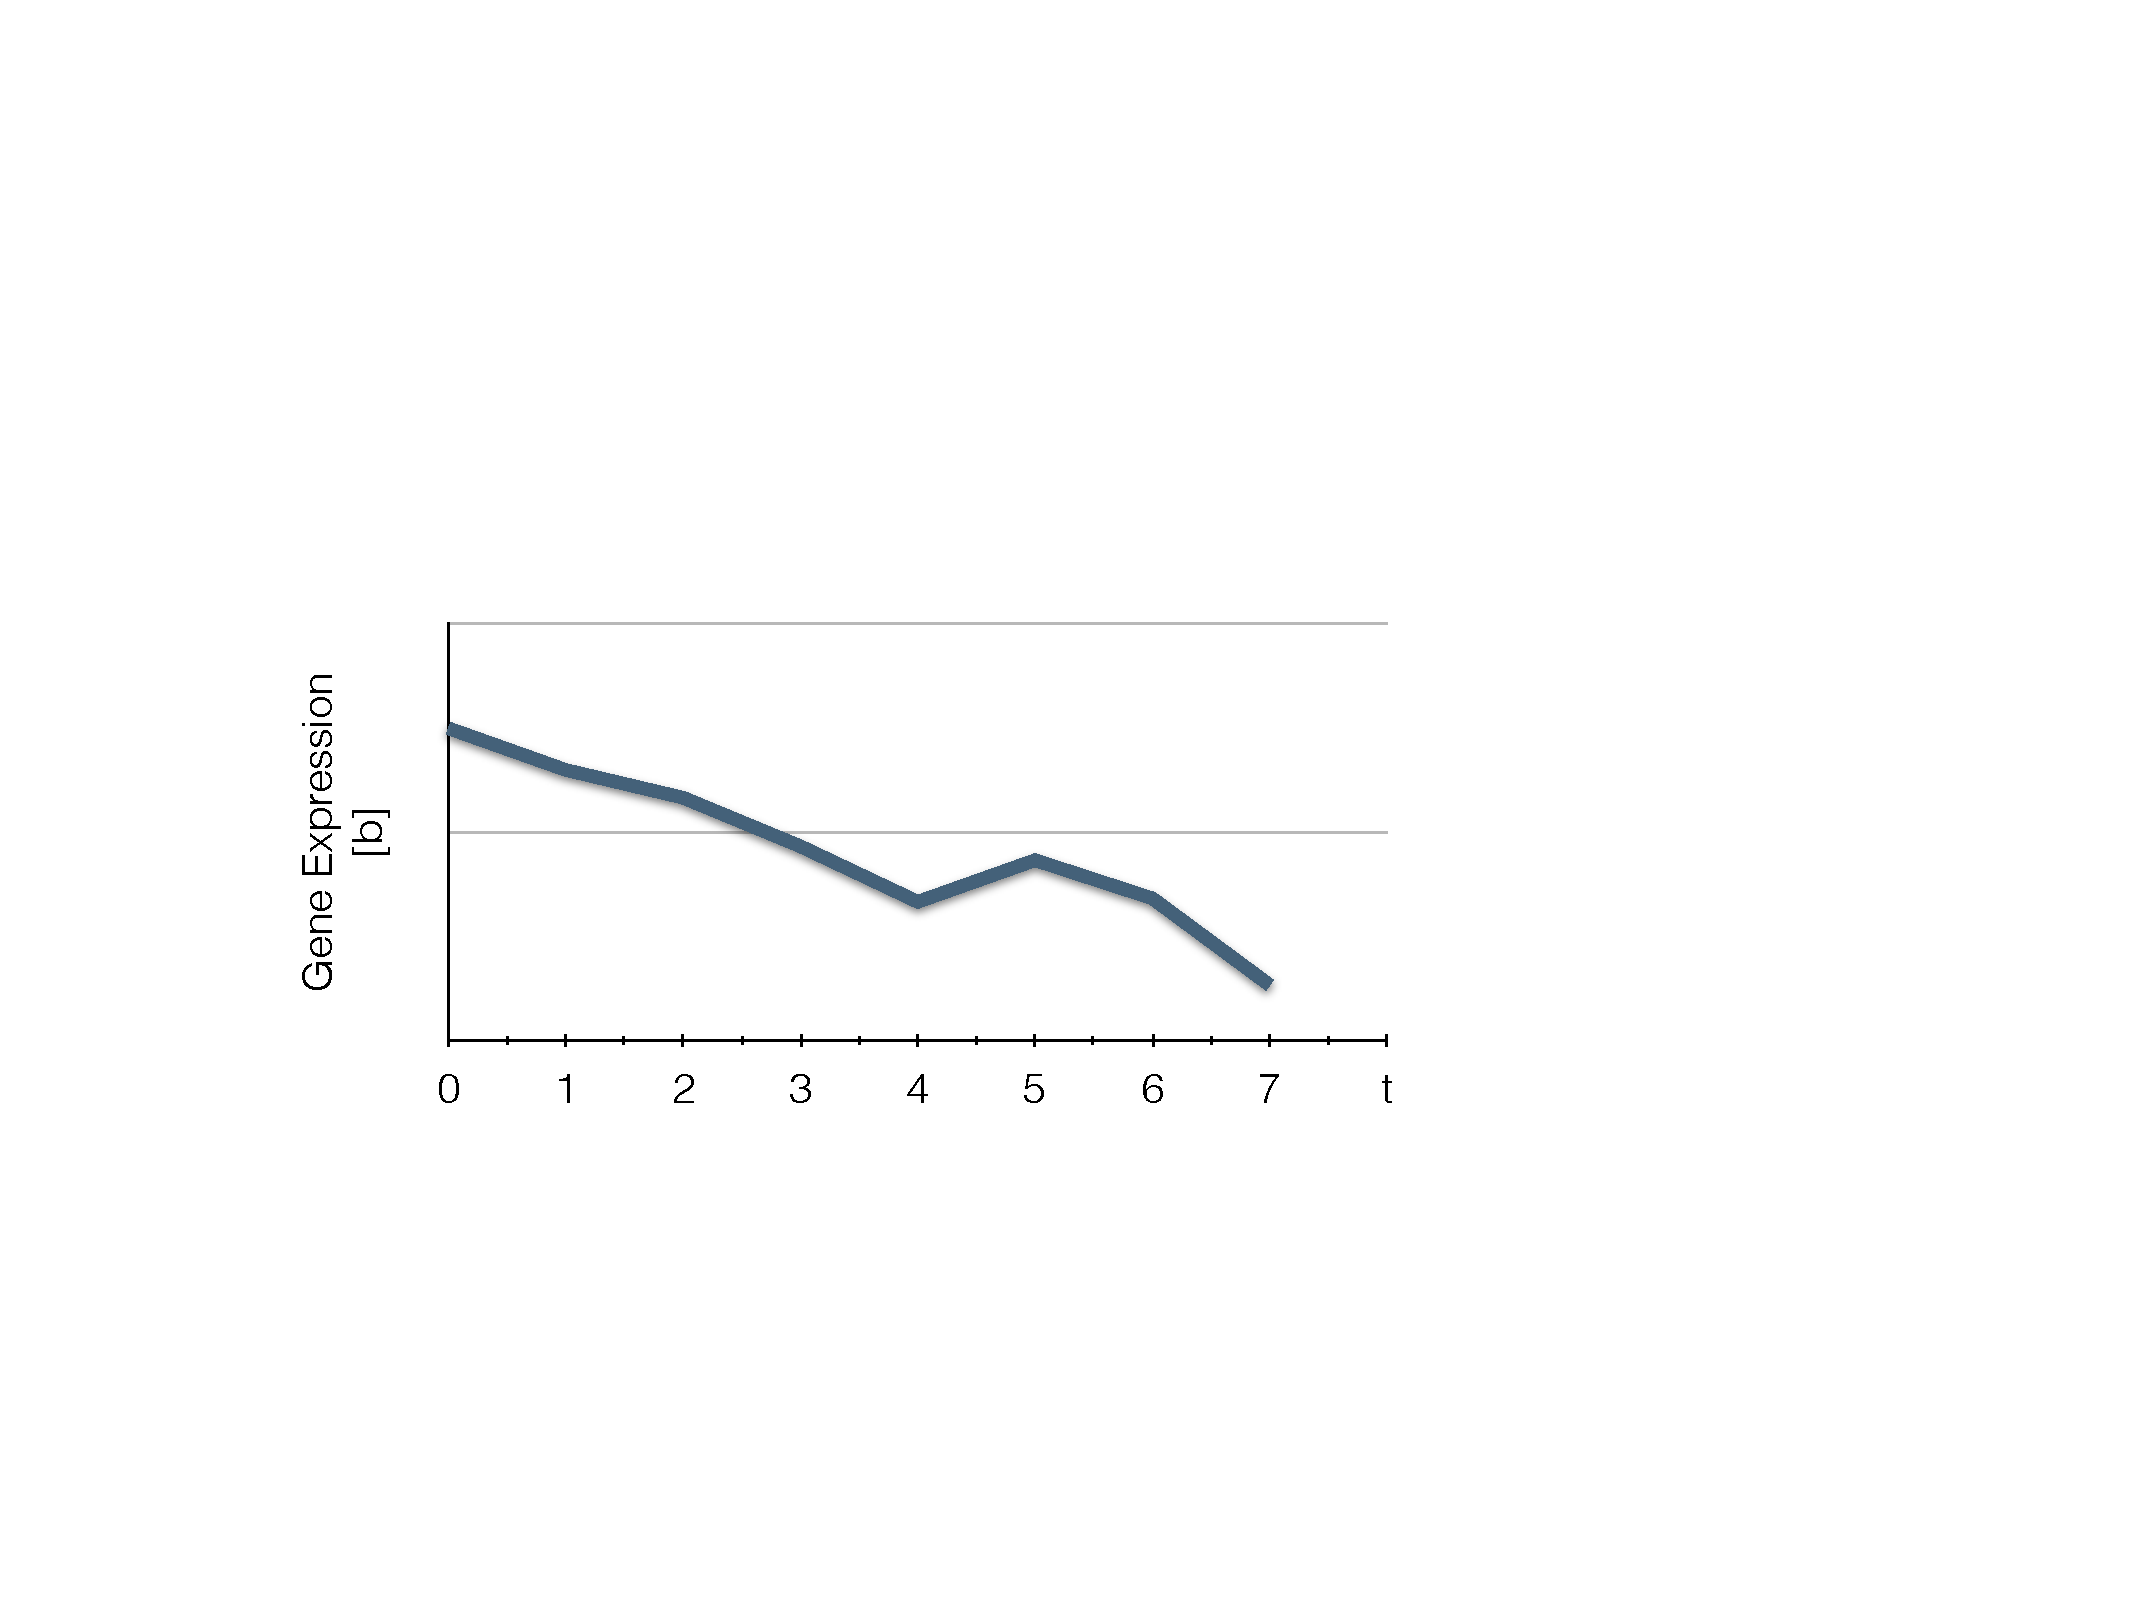
\includegraphics[ width =0.35\linewidth]{images/courbes/gene-b.pdf}\\
%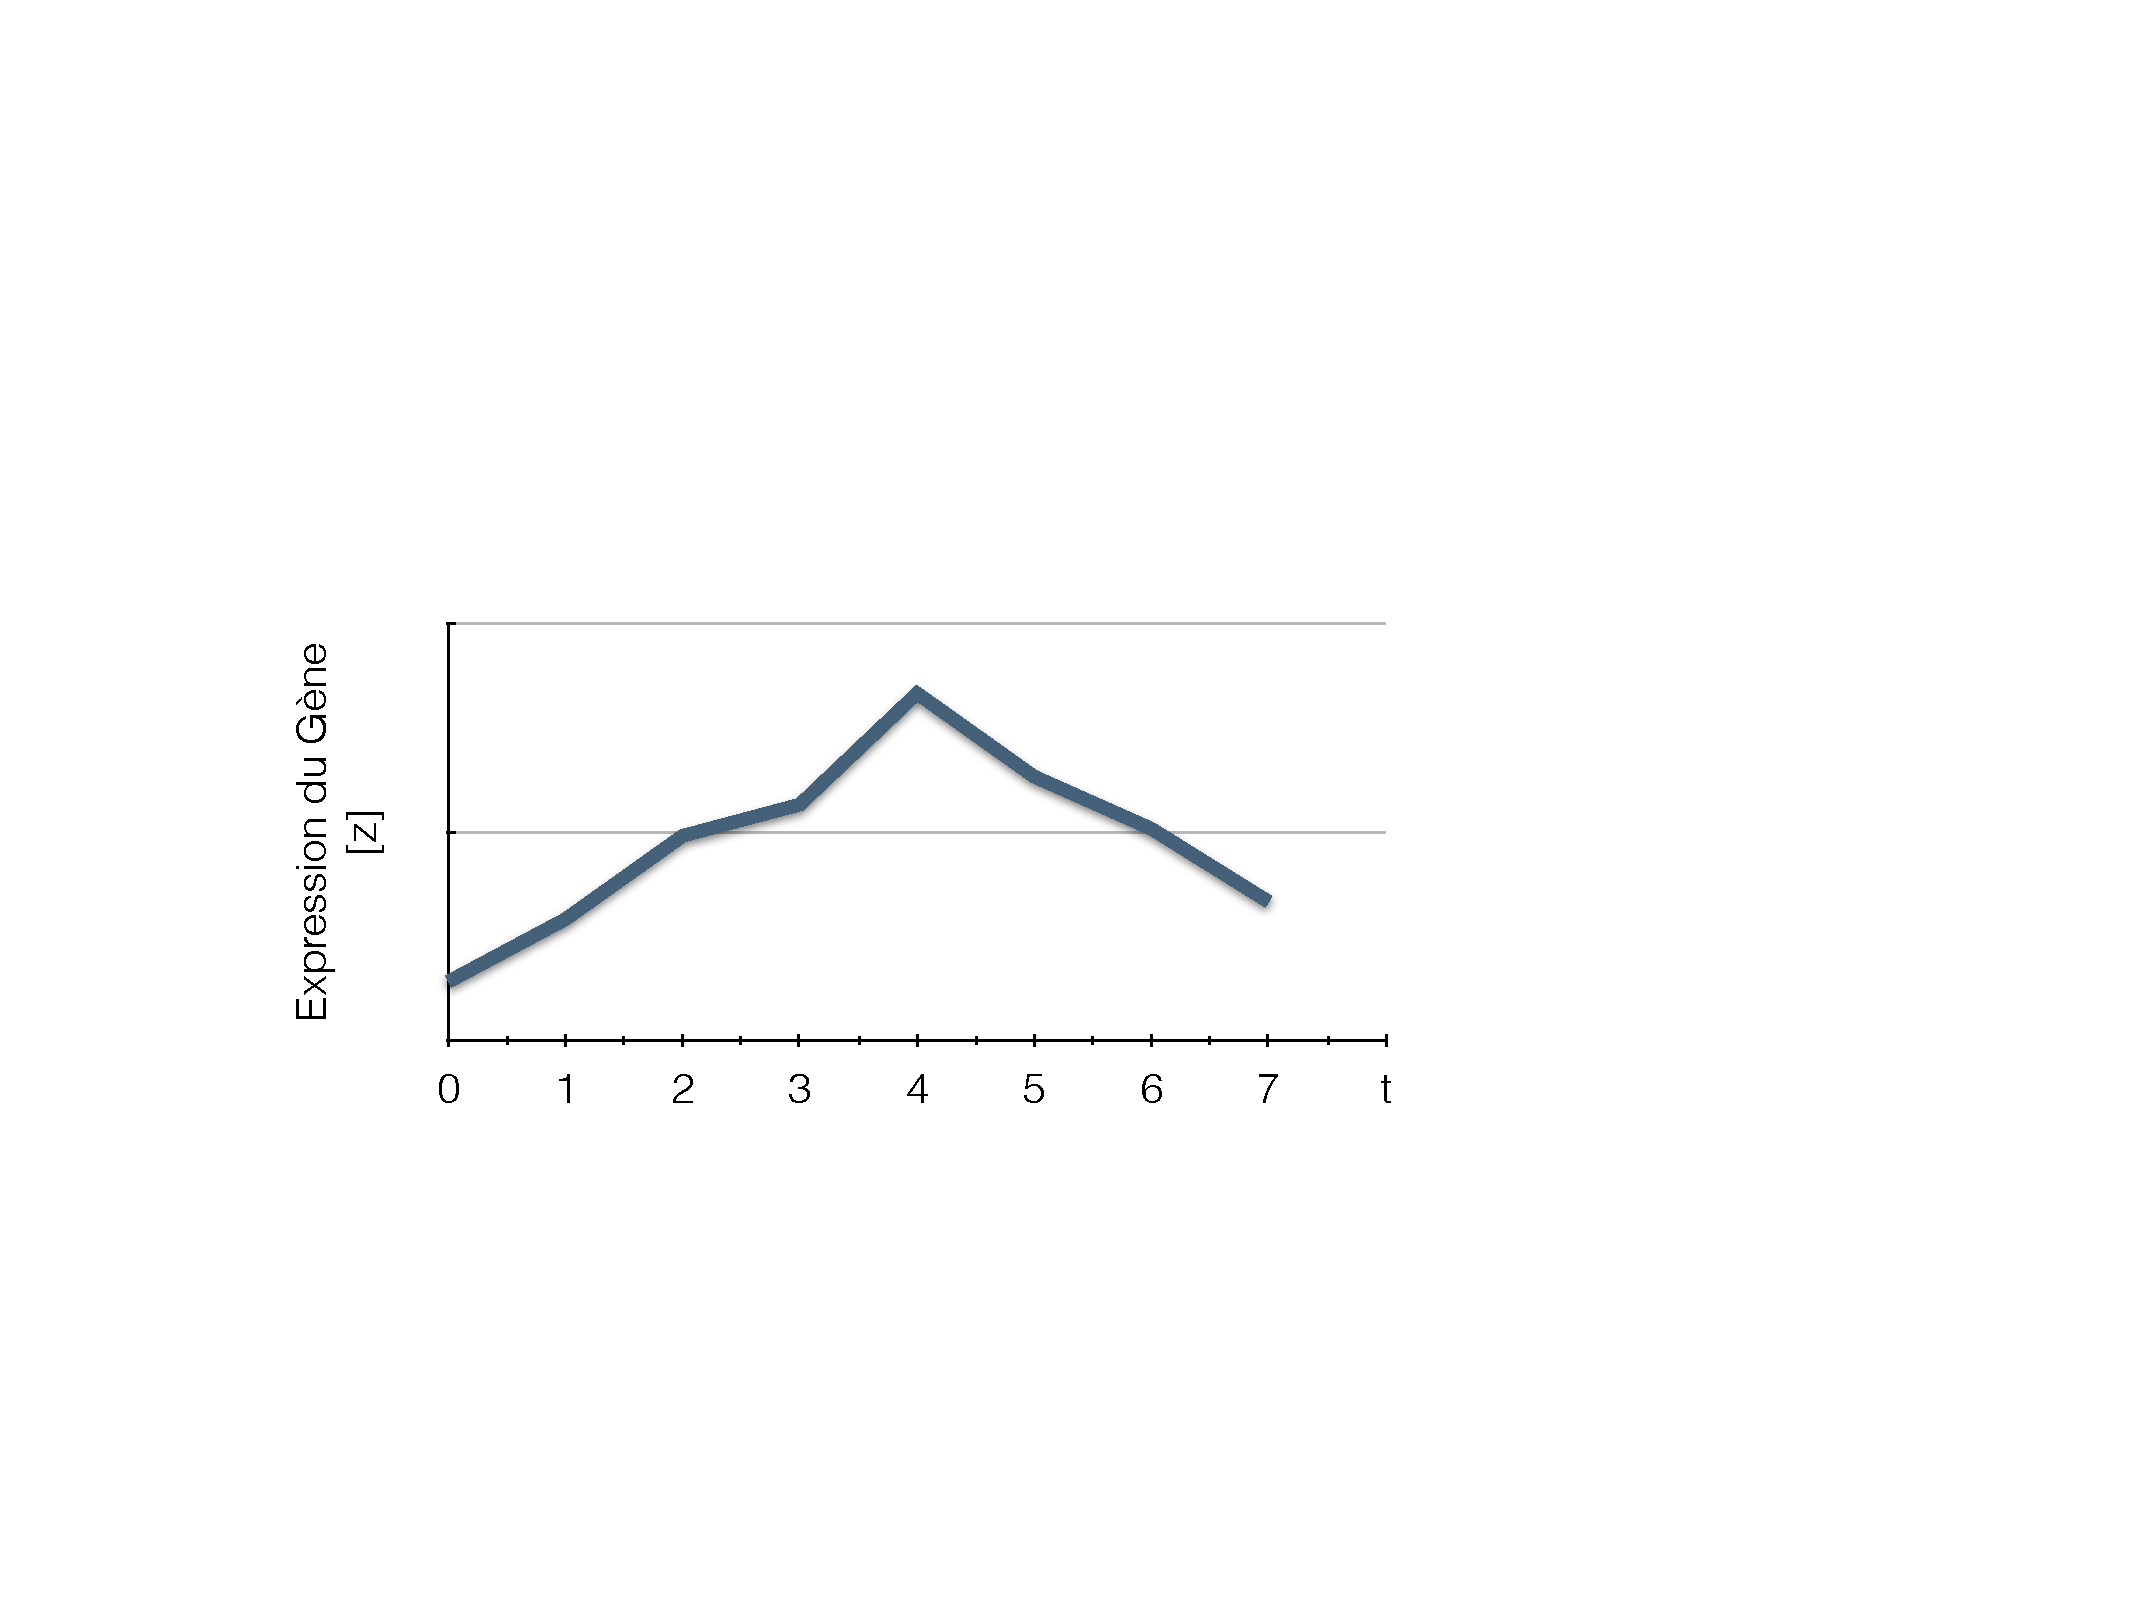
\includegraphics[ width =0.35\linewidth]{images/courbes/gene-z.pdf}
%\hspace{0.01cm}
%\textcolor{red}{$\Rightarrow$}
%\hspace{0.01cm}
%\begin{minipage}[t]{0.4\linewidth}
%\vspace{-5cm}
%Process Hitting:
%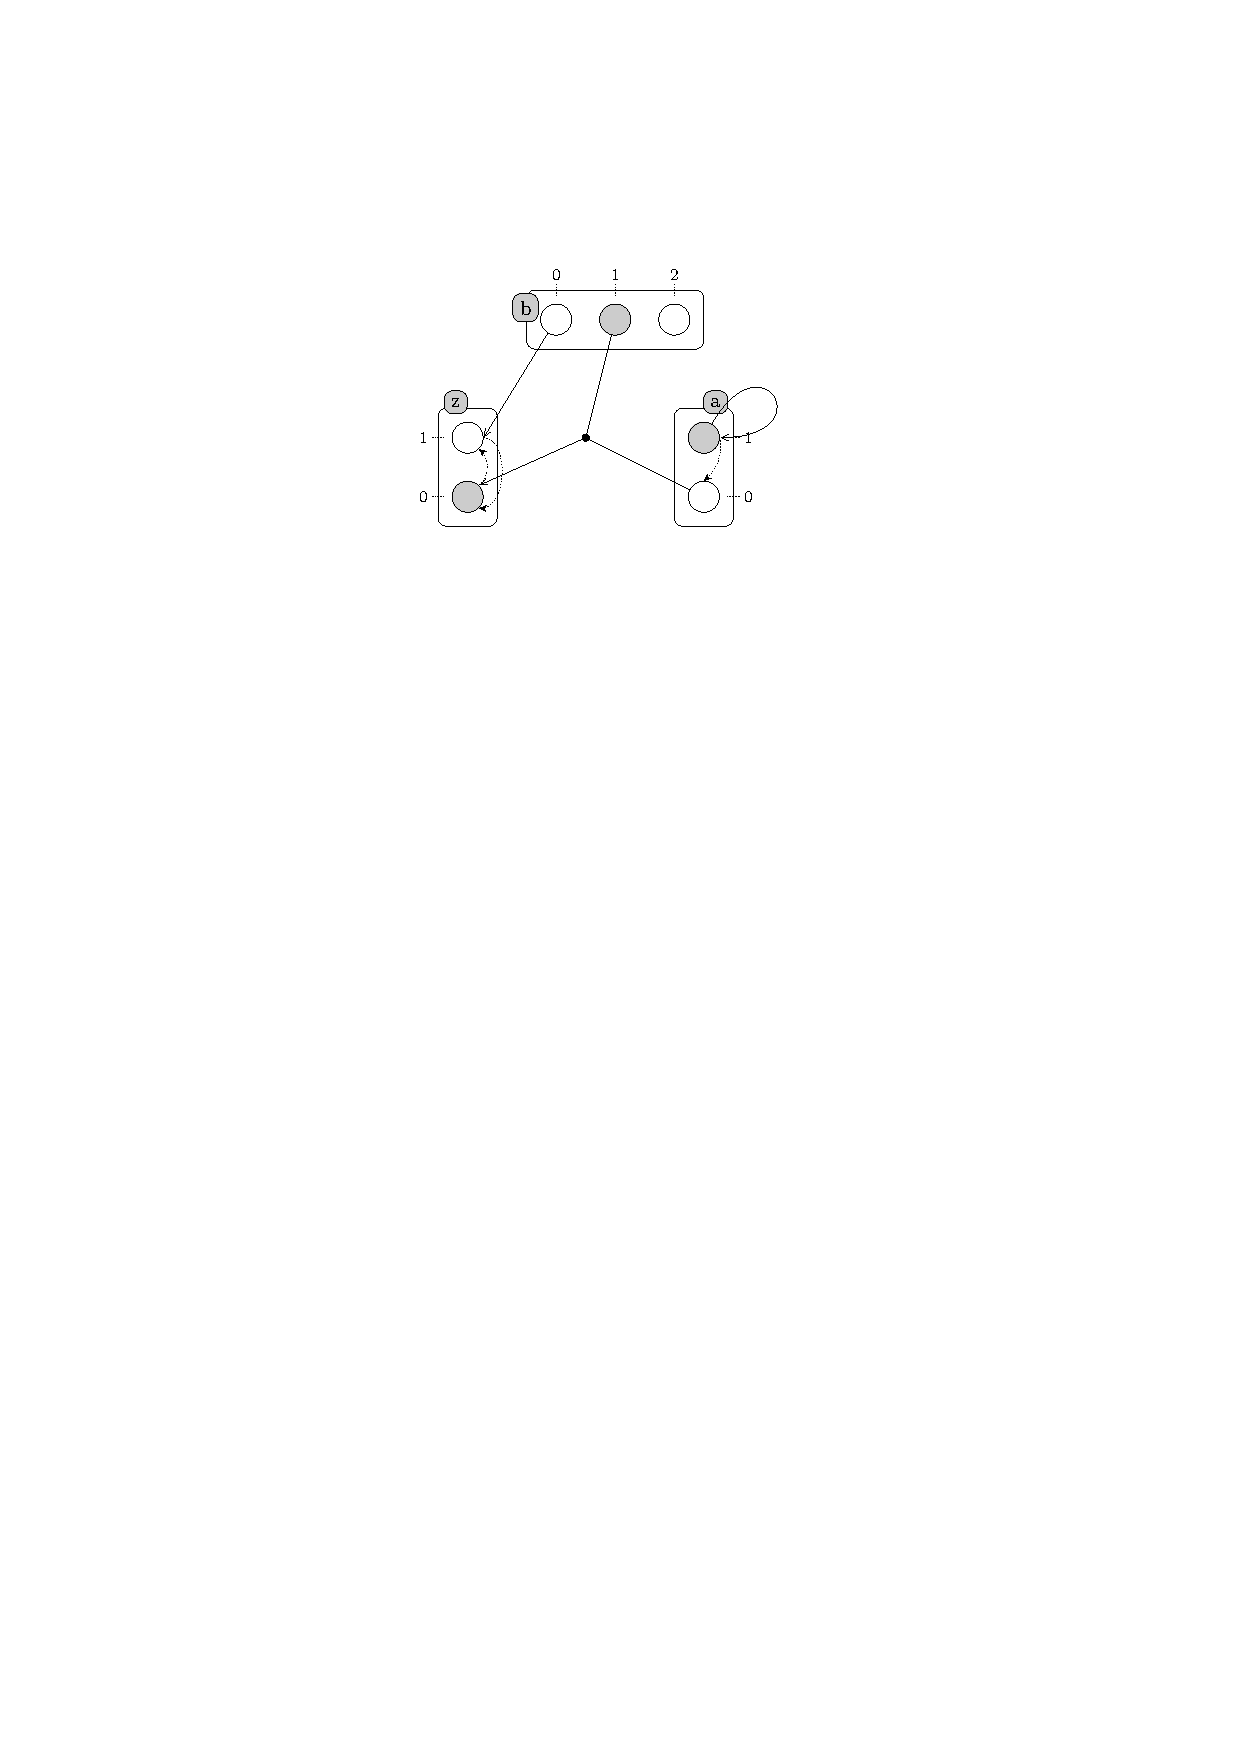
\includegraphics[width =1\linewidth]{images/PH-but.pdf}
%\end{minipage}
%\end{figure}


% Discretization figure
\begin{figure}[h]\centering
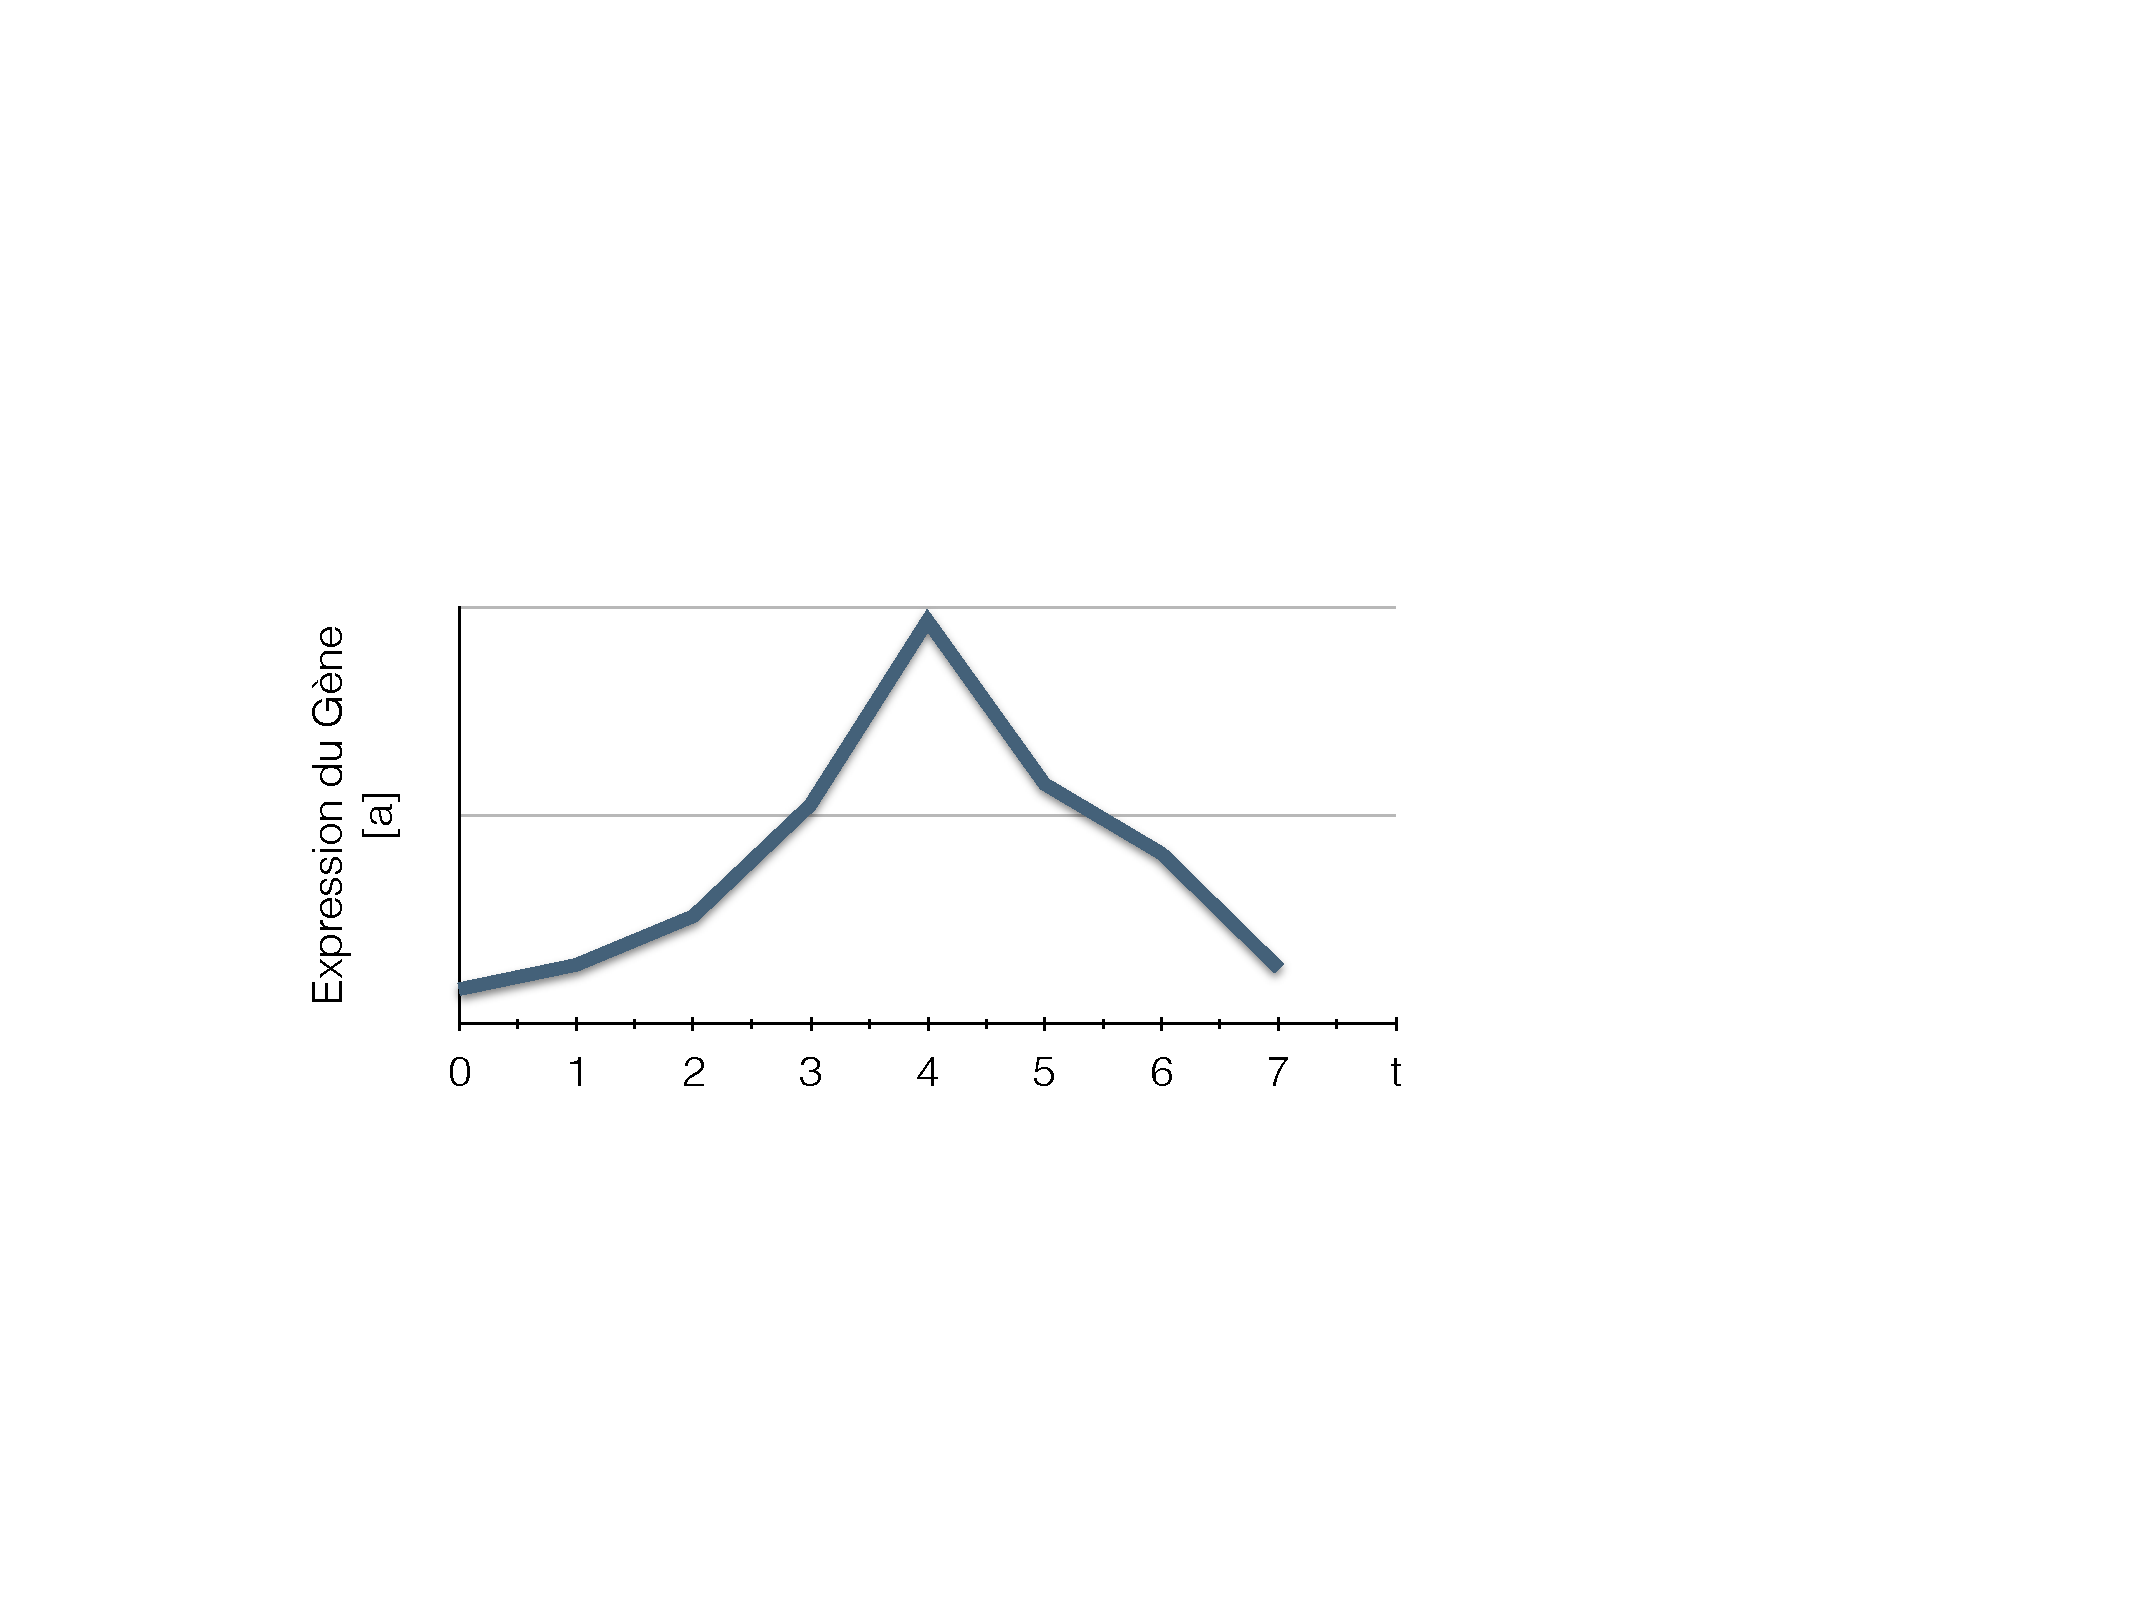
\includegraphics[width =0.31\linewidth]{images/courbes/gene-a.pdf}
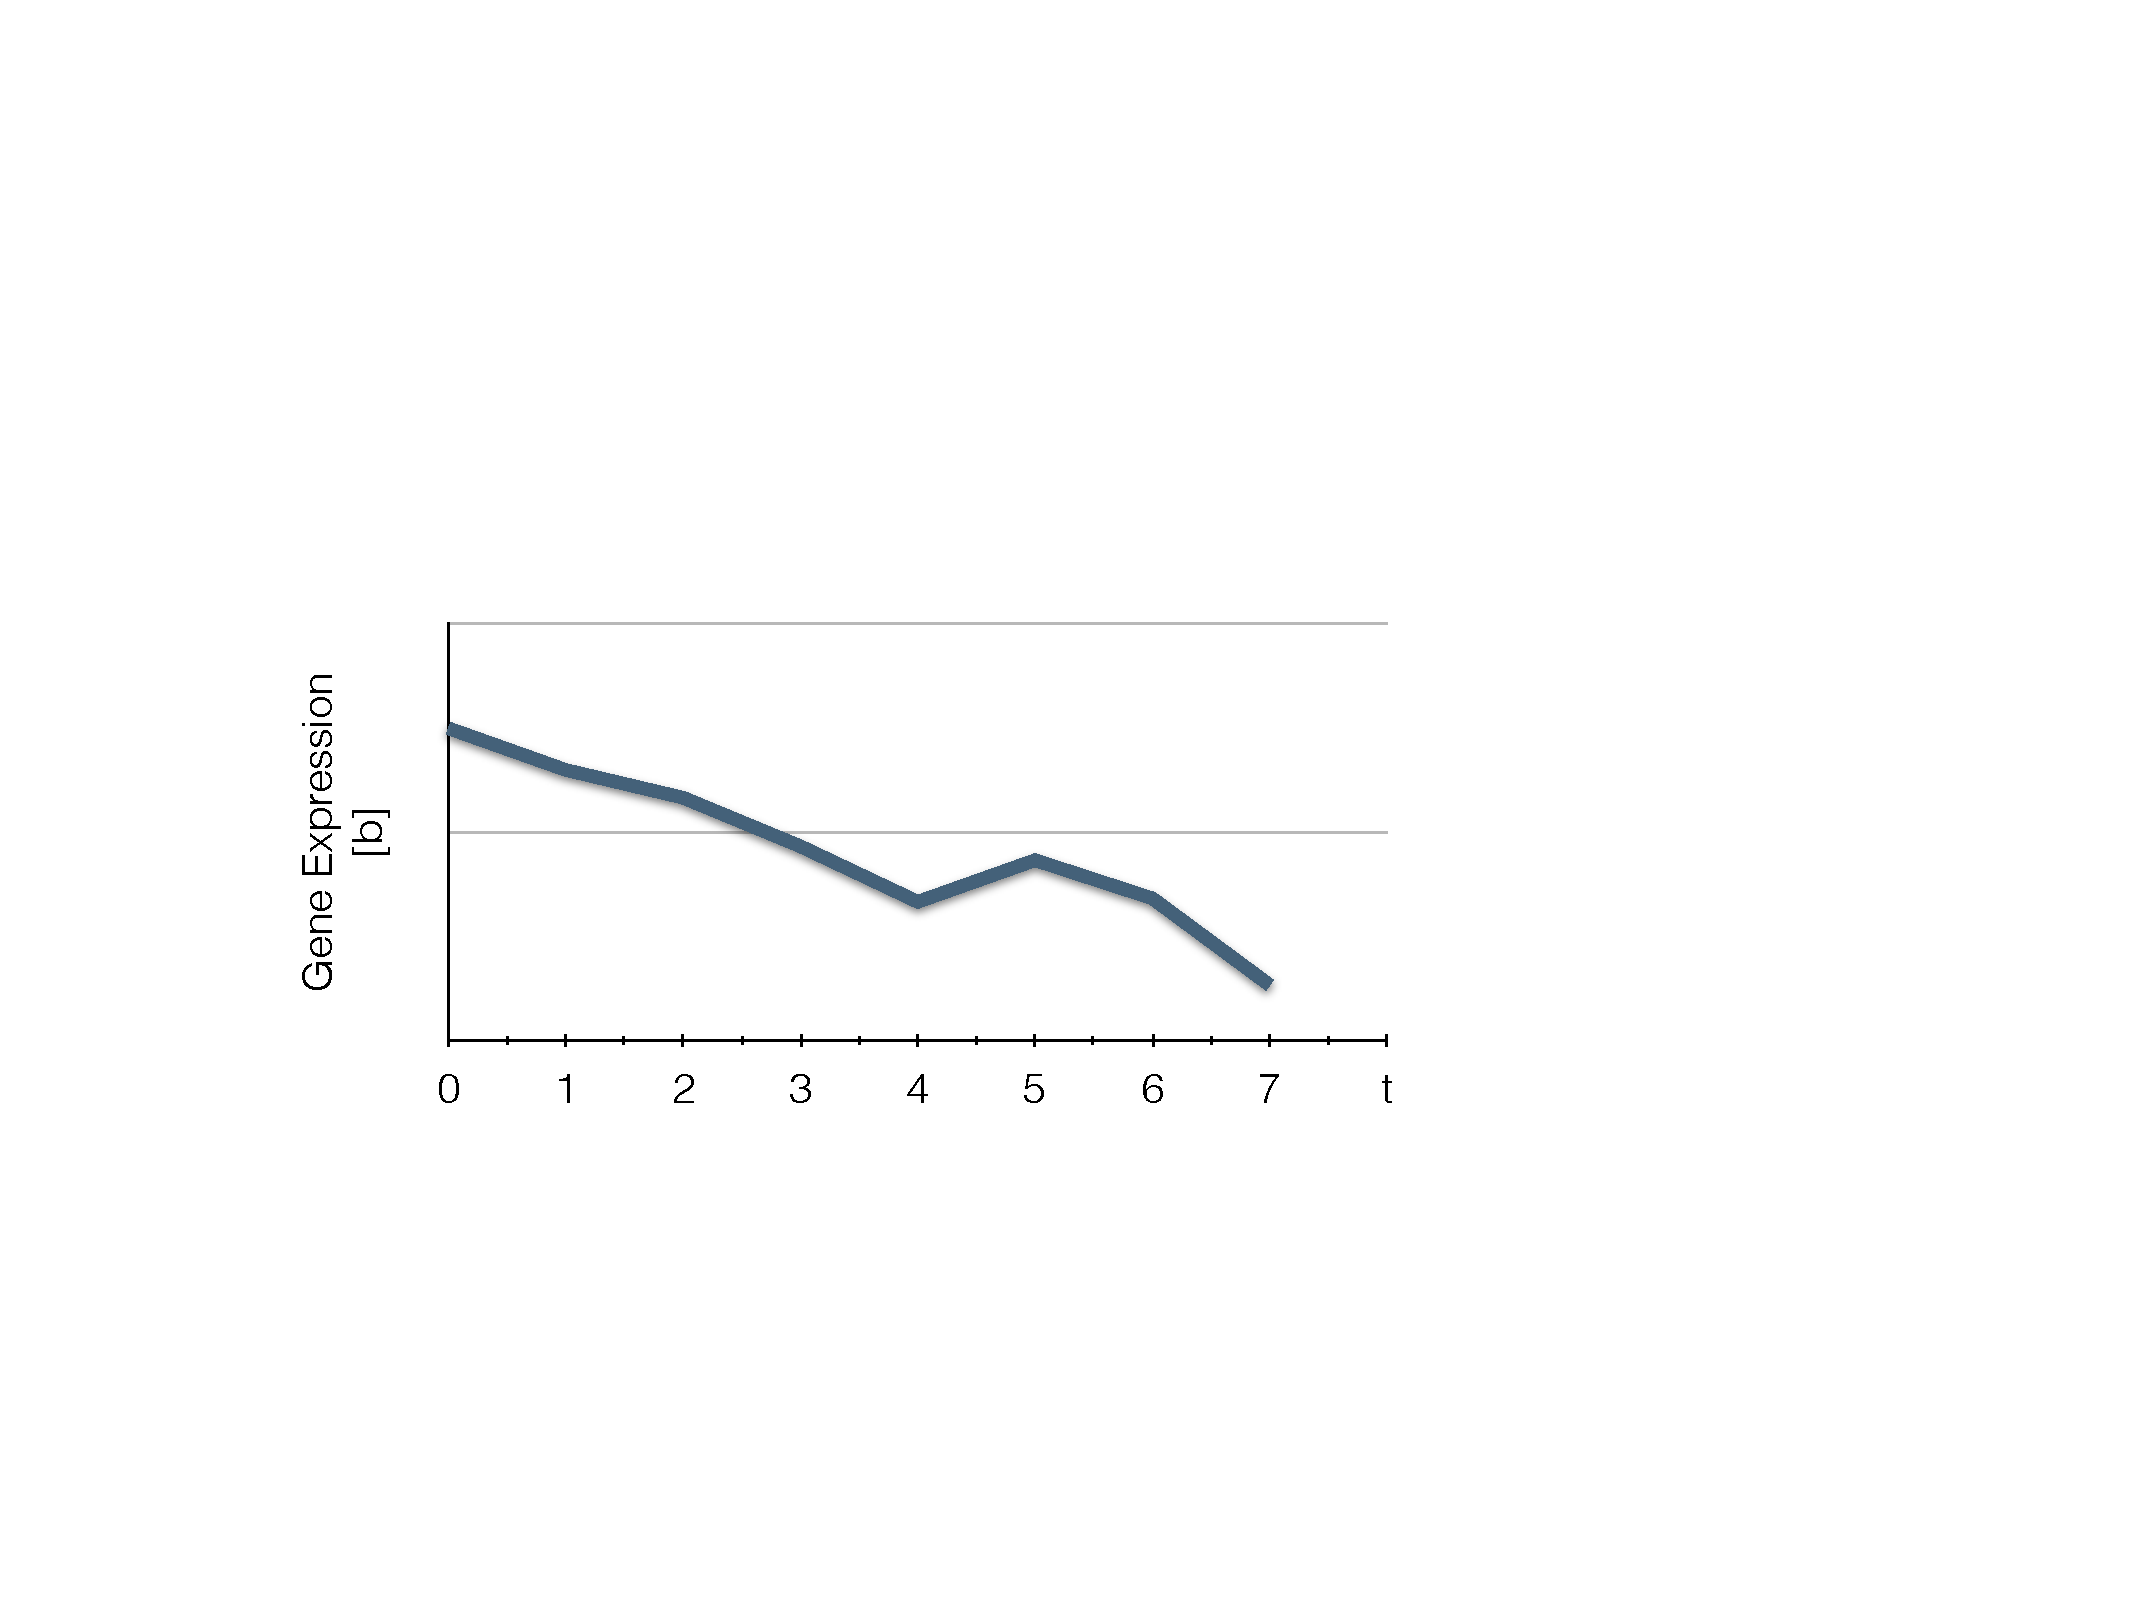
\includegraphics[width =0.31\linewidth]{images/courbes/gene-b.pdf}
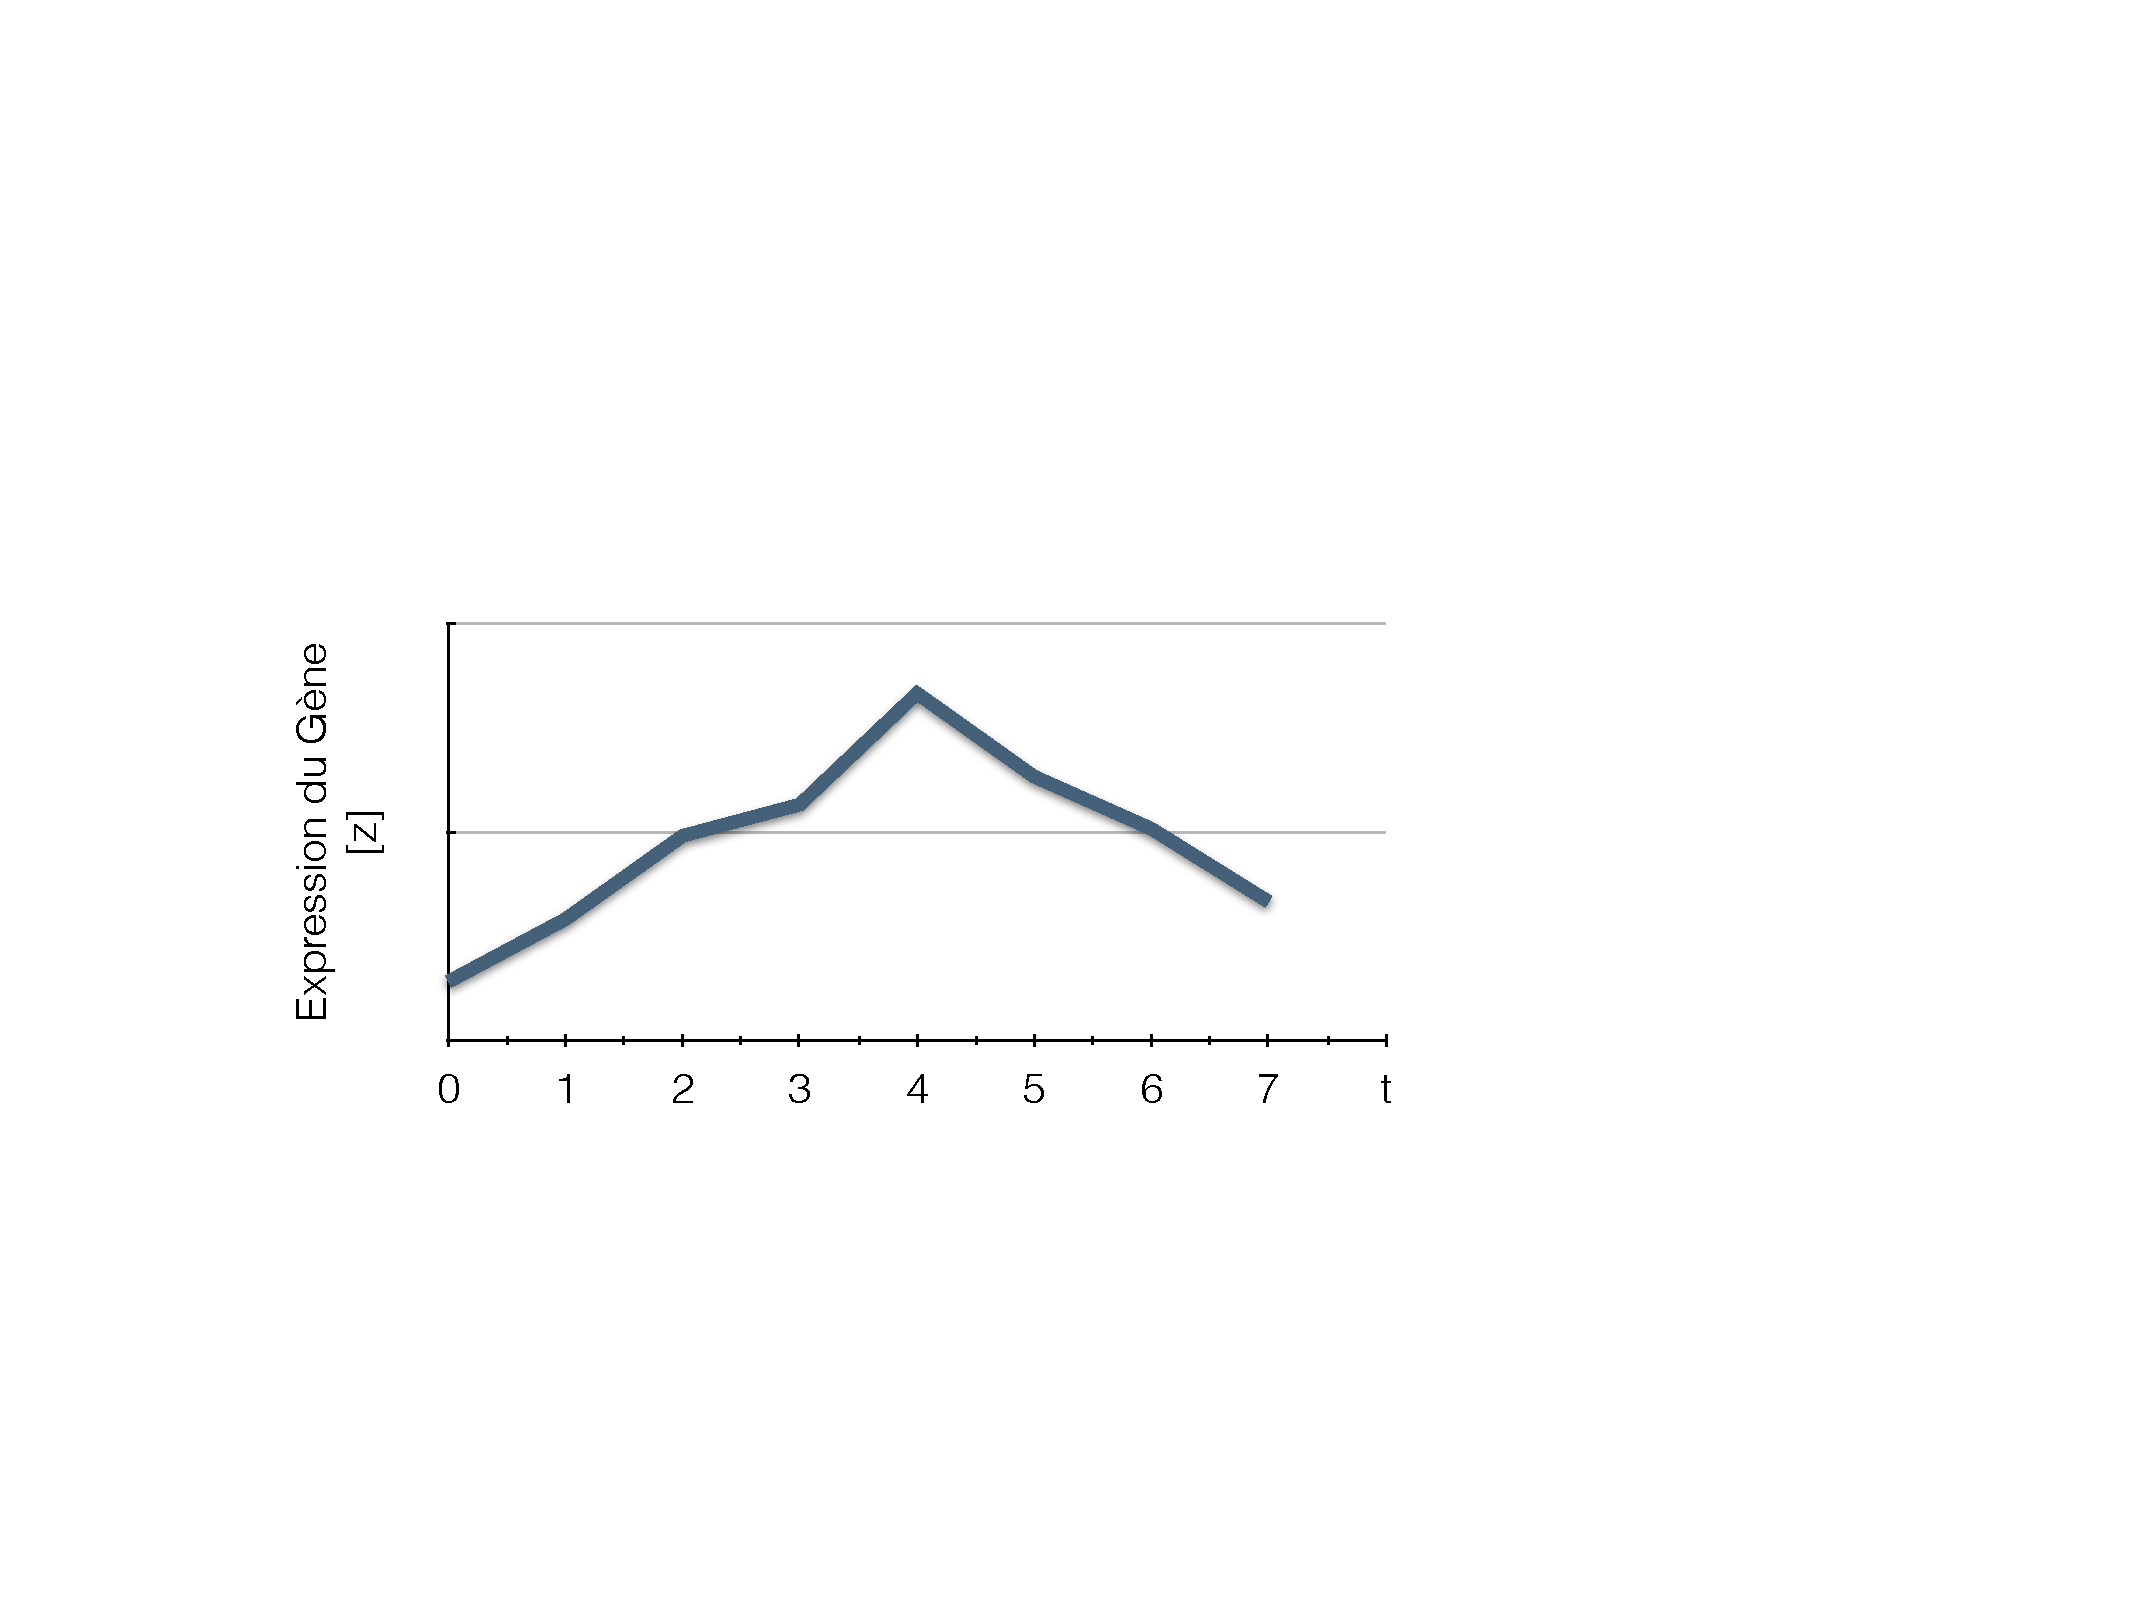
\includegraphics[width =0.31\linewidth]{images/courbes/gene-z.pdf}

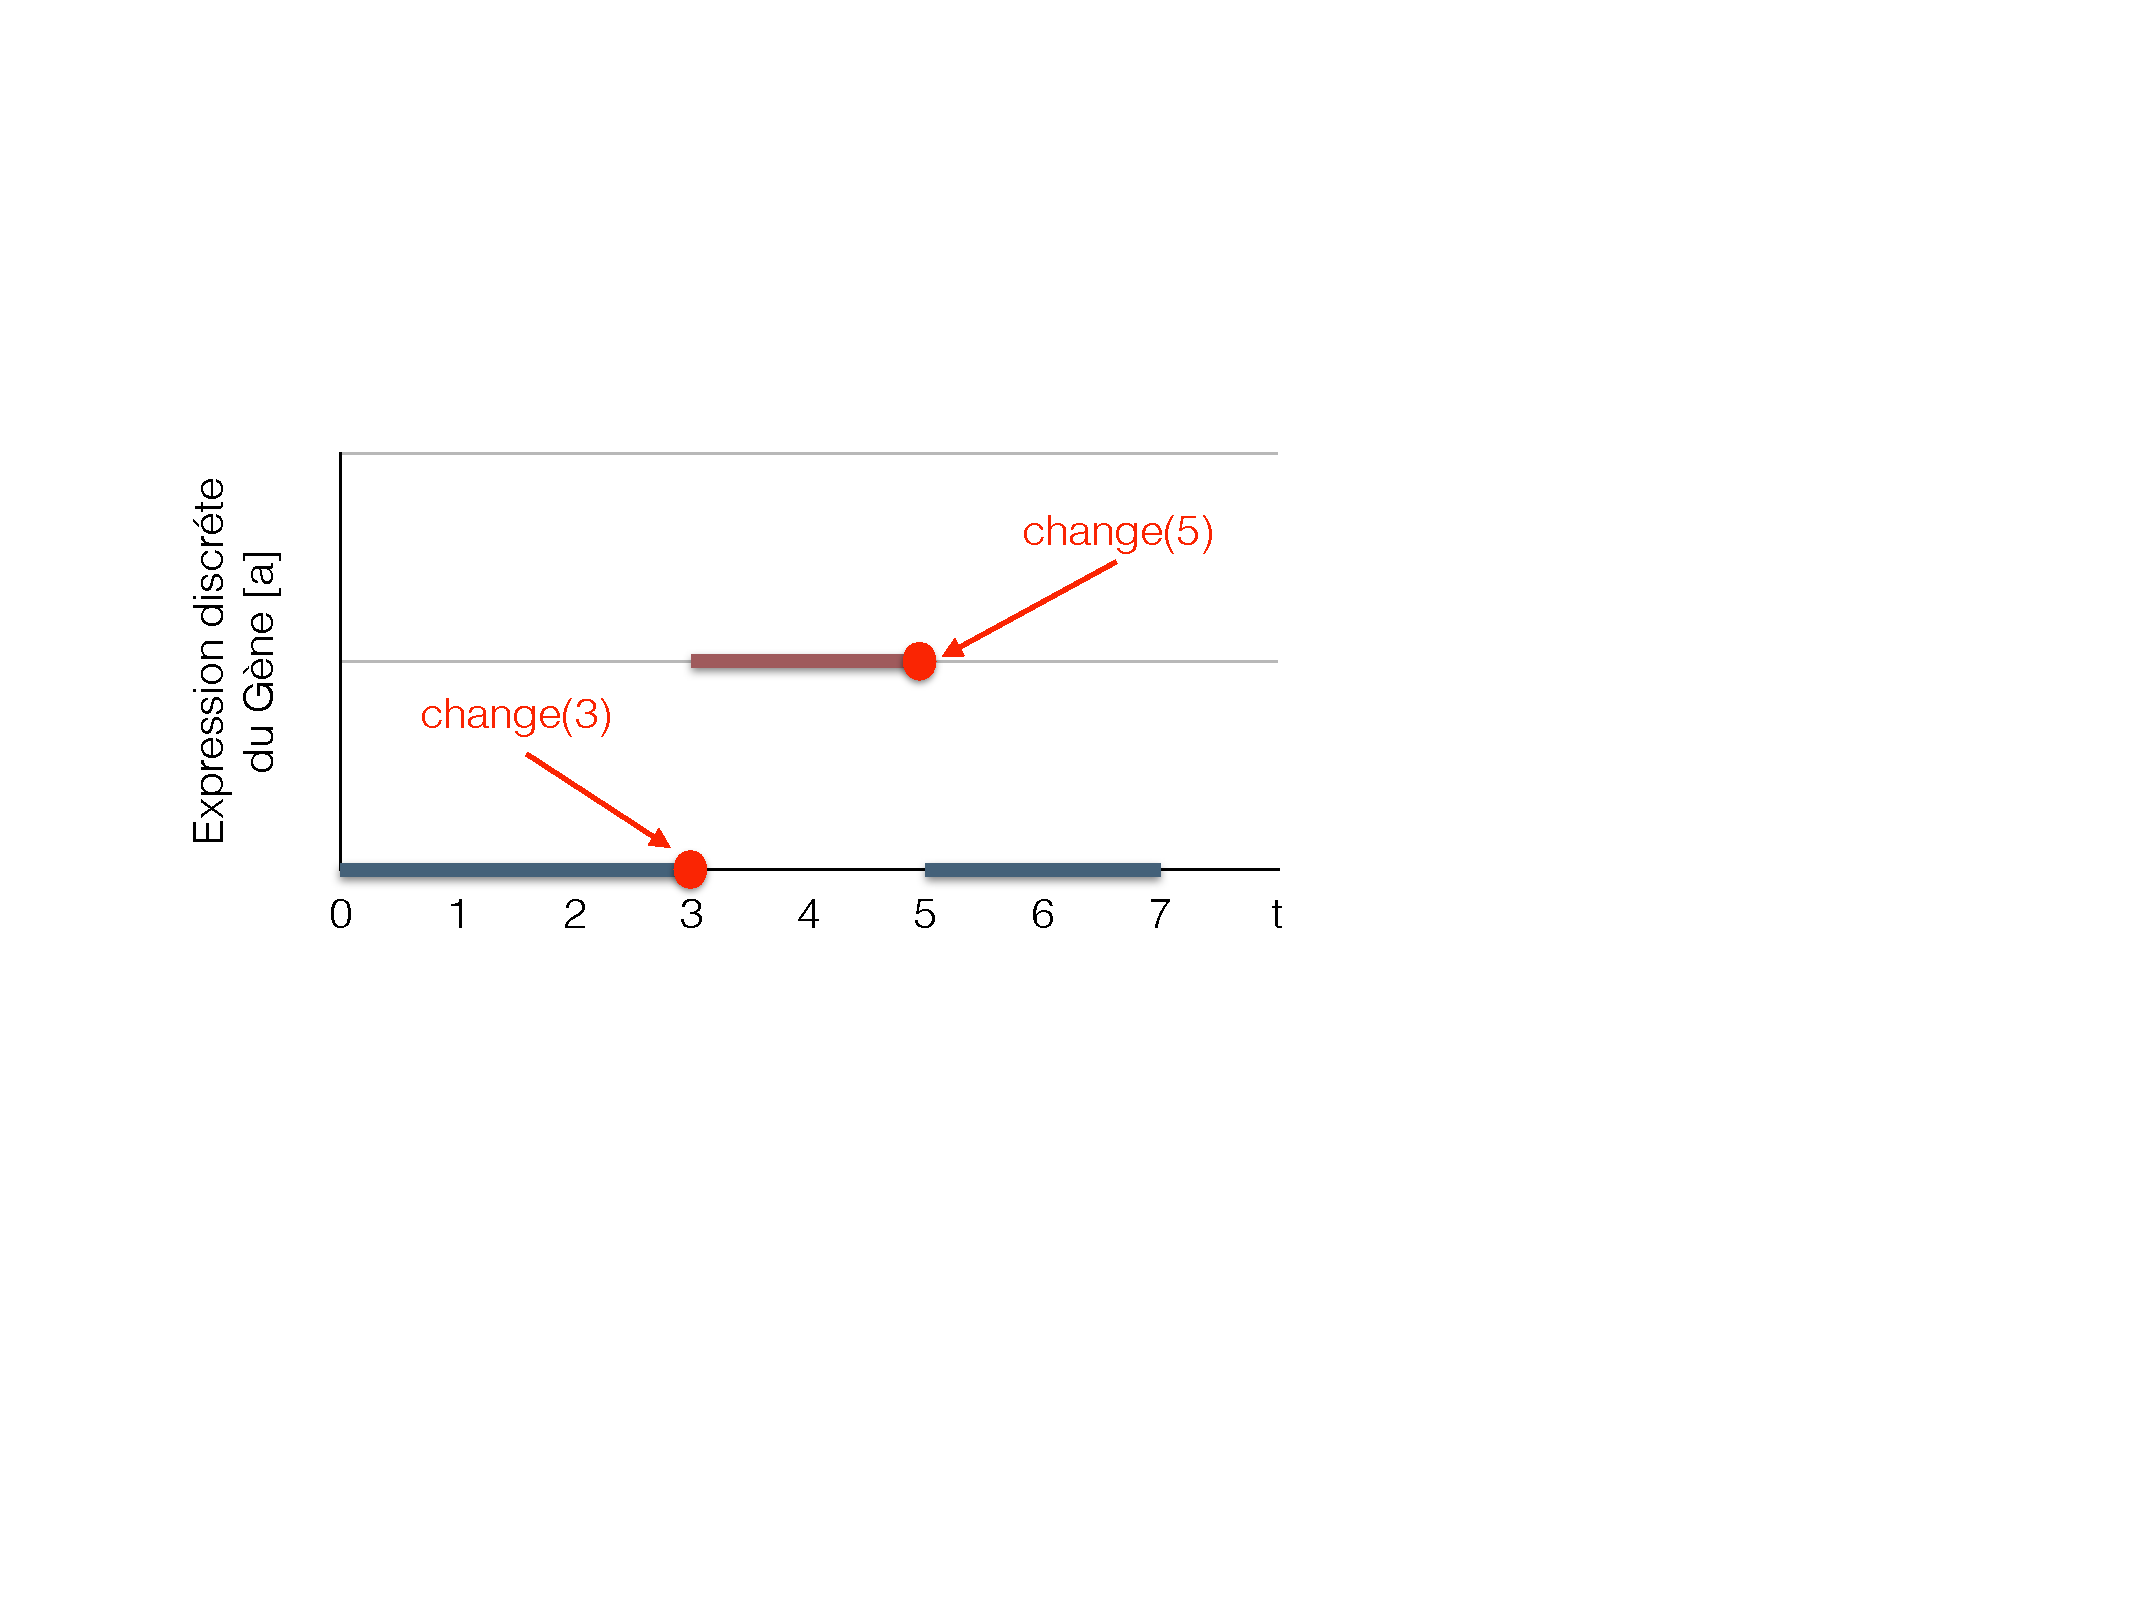
\includegraphics[width =0.31\linewidth]{images/courbes/gene-a-disc-change.pdf}
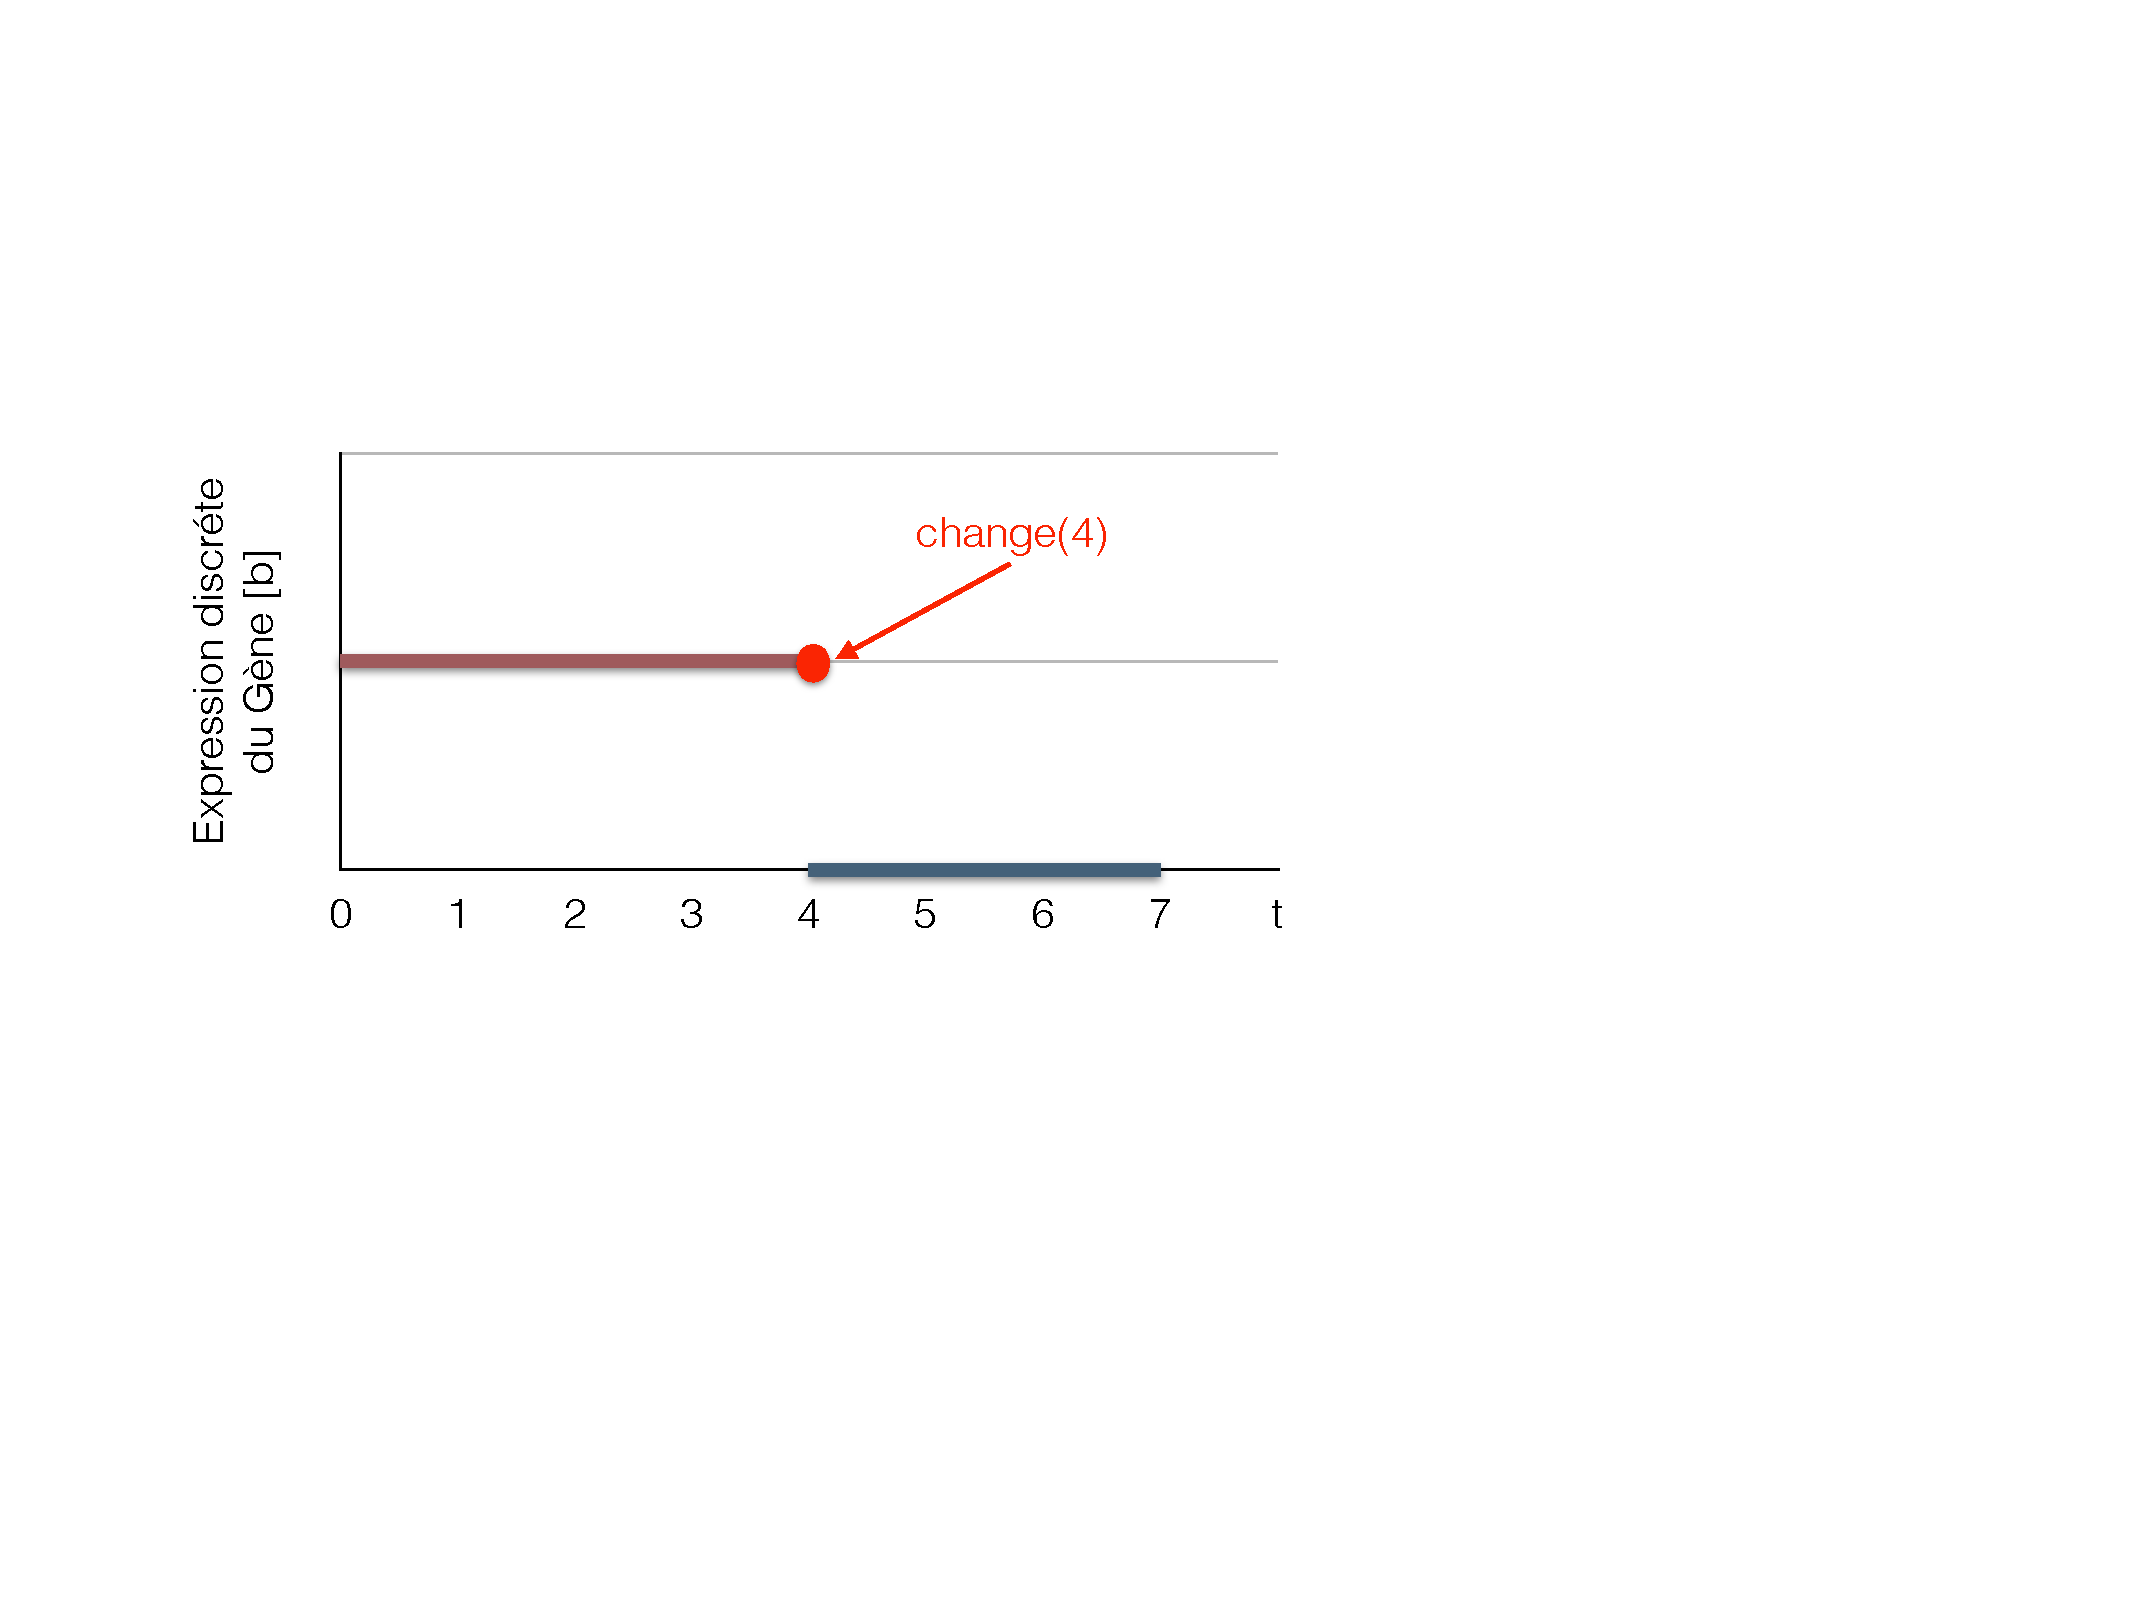
\includegraphics[width =0.31\linewidth]{images/courbes/gene-b-disc-change.pdf}
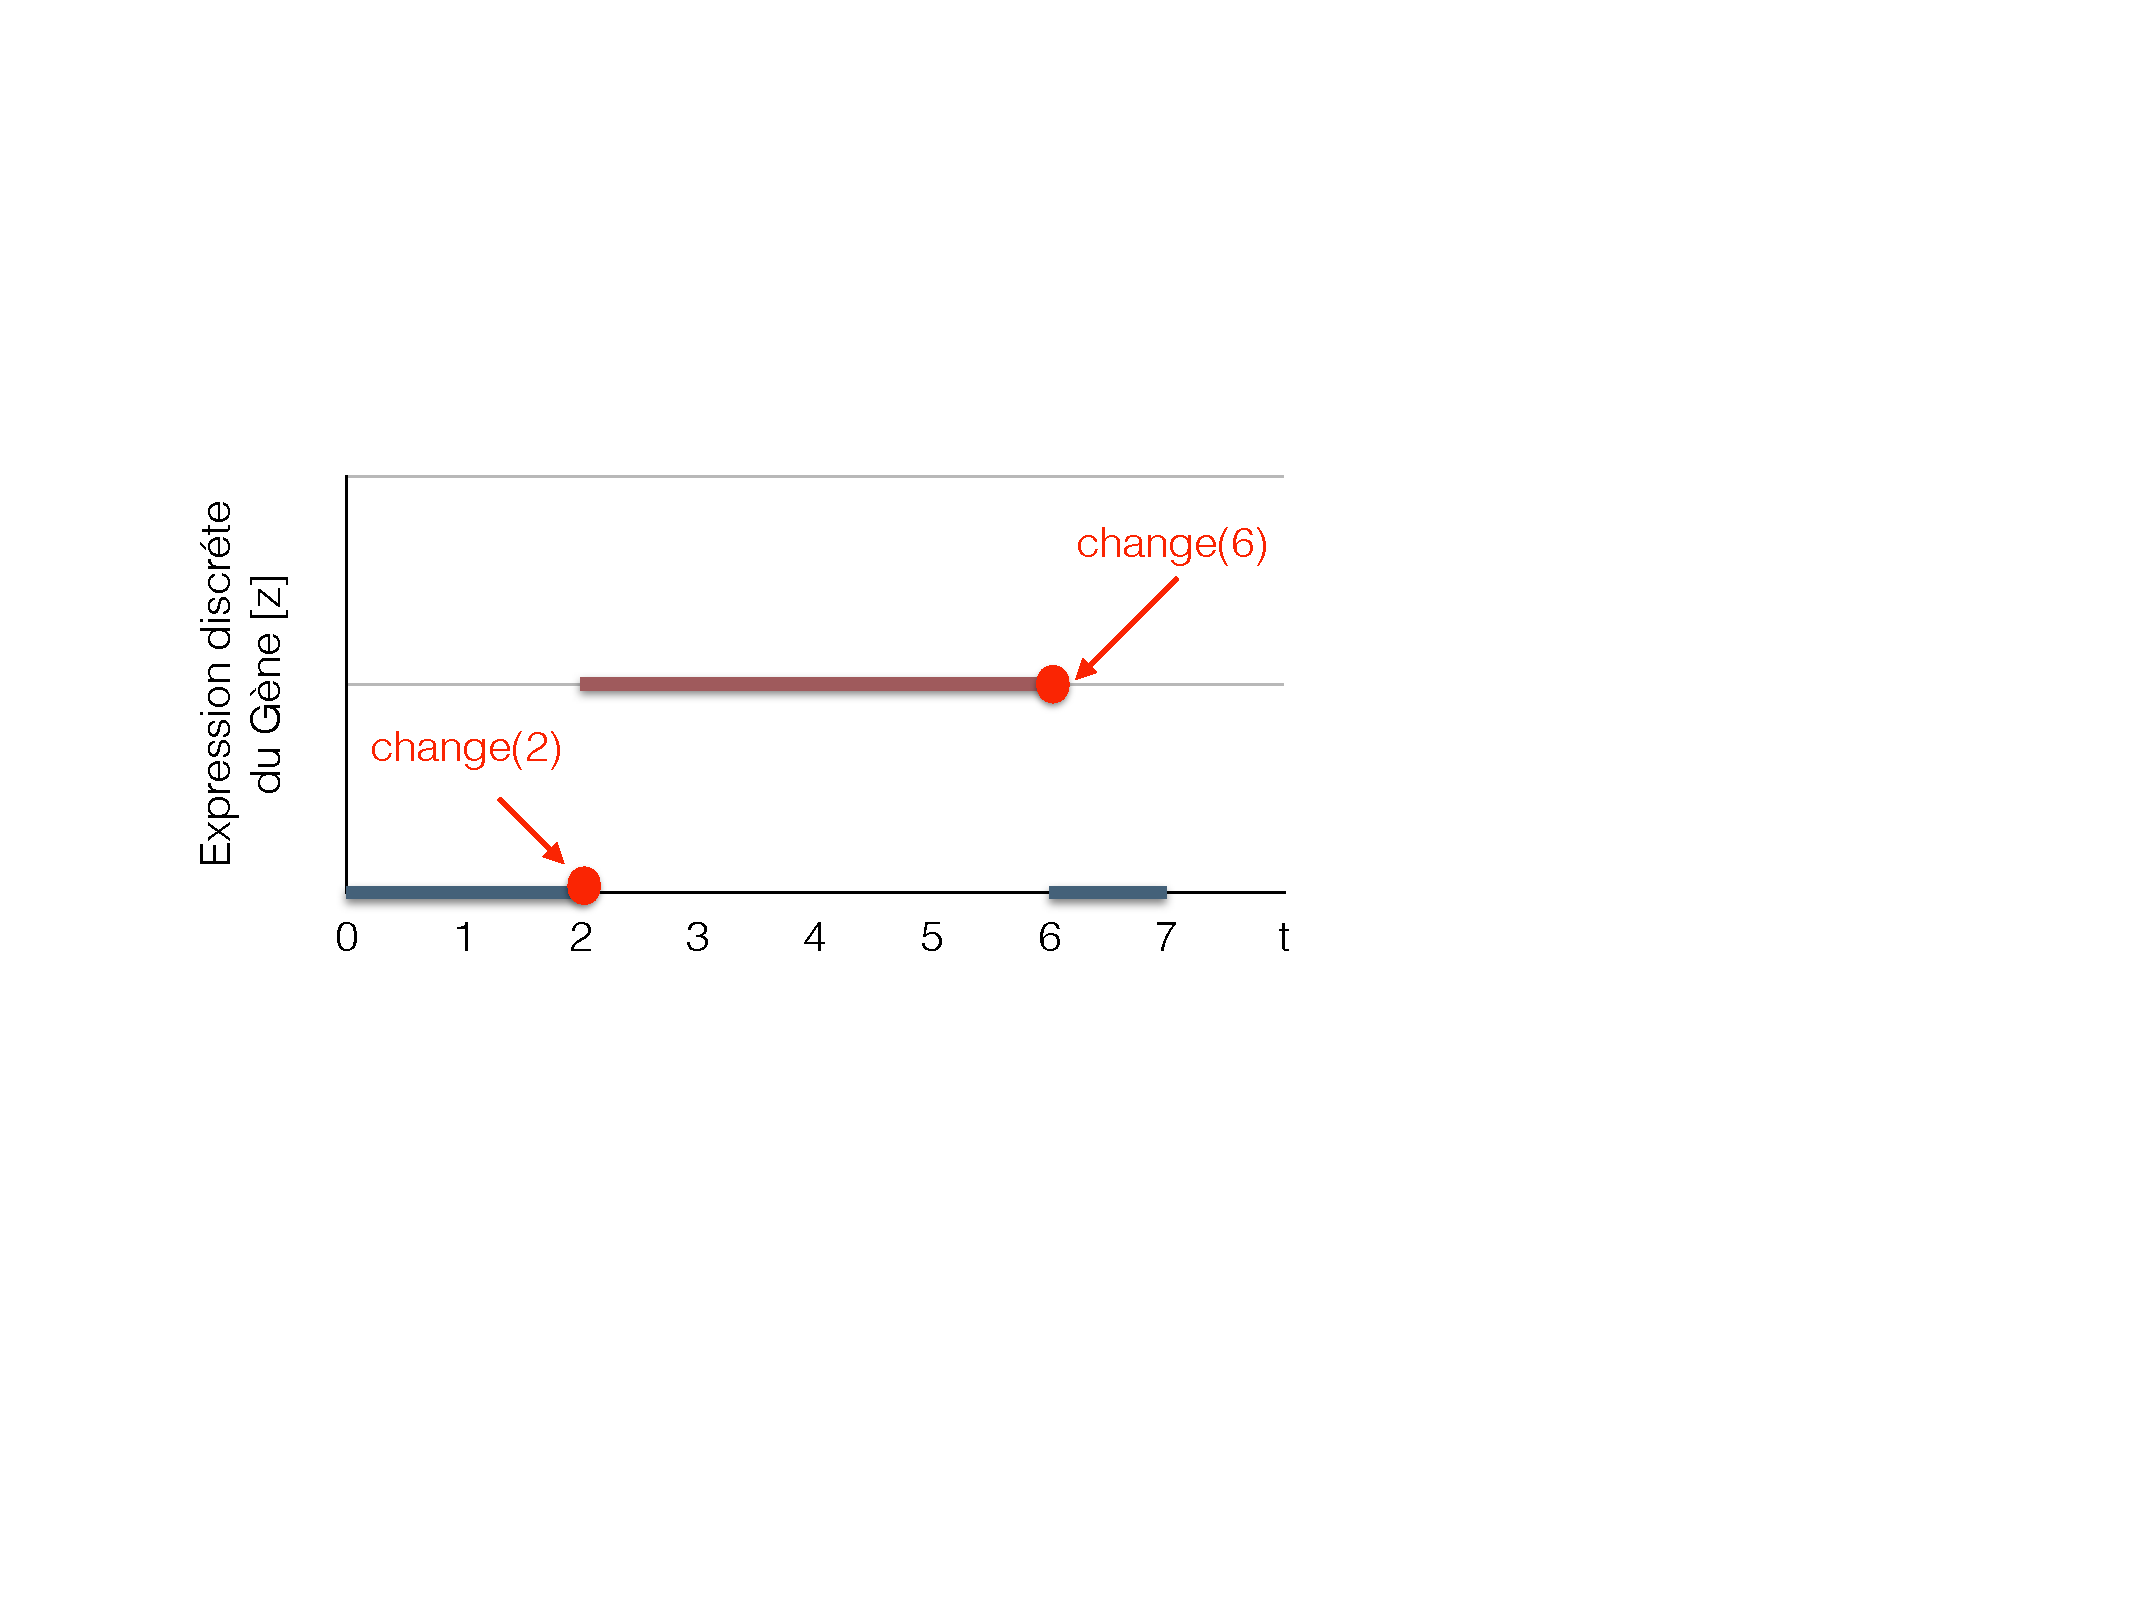
\includegraphics[width =0.31\linewidth]{images/courbes/gene-z-disc-change.pdf}
\caption{Examples of the discretization of continues time series data into bi-valued chronograms.
Abscisse represents time and ordinate the gene expression level.
The expression level is discretized according to a treshold fixed to the half of the gene expression value in this example.}
\label{fig:discretization}
\end{figure}

We can summarrize our method in the following steps:
\begin{itemize}
\item[-] Detection of changes
\item[-] Computation of the interactions possibly reponsible of thoses changes
\item[-] Filtering of the candidates actions
\item[-] Add actions to the model: completion/revision of the model
\end{itemize}

% Running example

We will now show an example of the execution of algorithm on the chronogram of Figure \ref{fig:discretization}:

%Let $i$ be the maximal number of hitters in an action of a PH: {\textit the indegree}.

The first change occurs at $t_1$ = $t_{min}$ = 2,
wich we will denote as \texttt{change(2)}.
It has been caused by an action $h = \PHfrappedelay{A}{D}{z_0}{z_1}$
where $ A \in \PHl^{\diamond}, | A| \leq i, i=2$ and $D$ is the delay wich is equal to 2 here since
$D_{t_i}=t_i - t_{i-1}$, such that $\exists$ \texttt{change($t_i$)} and \texttt{change($t_{i-1}$)},
$D_{t_1}= t_1 - t_0 = 2 - 0 = 2$.

Let $R=\{ b \rightarrow z, a \rightarrow z, a \rightarrow a \}$
be the set of regulation influences amoung the components of the system.
%
In the first change $t_1$ = 2 that we will denotes as $change(2)$,
its \texttt{z} whose value changes from $z_0$ to $z_1$, thus the action that has realized this change is of the form $h = \PHfrappedelay{A}{2}{z_0}{z_1}$. According to $R$ the genes which influence \texttt{z} are $G_{R_z} = \{\texttt{a, b}\}$. It means that $A= \{ a_{\textcolor{red}{?}}, b_{\textcolor{red}{?}} \} $ or $A= \{ a_{\textcolor{red}{?}} \} $ or $A= \{ b_{\textcolor{red}{?}} \} $
%
The expression level of the genes of $G{R_z}$ between $t_i$ and $t_{i-1}$ is as follows:
\begin{itemize}
\item[-] $a \in  G{R_z}$: $[a]_t=0$ $\forall t \in [0,2] $
\item[-] $b \in  G{R_z}$: $[b]_t=1$ $\forall t \in [0,2] $
\end{itemize}
%
Thus $A= \{ a_0, b_1 \} $ or $A= \{ a_0\} $ or $A= \{ b_1 \} $ and the set of candidate actions is:
$H_{change(2)} = \{ h_1=\PHfrappedelay{a_0}{2}{z_0}{z_1}
, h_2=\PHfrappedelay{b_1}{2}{z_0}{z_1}
, h_3=\PHfrappedelay{a_0 \wedge b_1 }{2}{z_0}{z_1} \}$.

The second change occurs at $t_2$ = 3 and we will denotes it as $change(3)$.
Here its \texttt{a} whose value changes from $a_0$ to $a_1$, thus the action that has realized this change is of the form
$h = \PHfrappedelay{A}{\textcolor{red}{D}}{a_0}{a_1}$ 
where $ A \in \PHl^{\diamond}, | A| \leq 2$ and $D$ is the delay that is equal to 1 here: 
$D_{t_2}= t_2 - t_1 = 3 - 2= 1$
According to $R$ the genes which influence \texttt{a} are $G_{R_a} = \{\texttt{a}\}$.
It means that $A= \{ a_{\textcolor{red}{?}}\}$ and the expression level of \texttt{a} between $t_1$ and $t_{2}$ is $a_0$.
Thus  $A= \{ a_0\} $ and there is only one candidate action that is a self action:
$H_{change(3)} = \{ h=\PHfrappedelay{a_0}{1}{a_0}{a_1}  \}$.

The third change occurs at $t_3$ = 4 and we will denotes it as $change(4)$.
Here its \texttt{b} whose value changes from $b_1$ to $b_0$, thus the action that has realized this change is of the form 
$h = \PHfrappedelay{A}{D}{b_1}{b_0}$ where $ A \in \PHl^{\diamond}, | A| \leq 2$ and $D$ is the delay that is equal to 1 here:
$D_{t_3}= t_3 - t_2 = 4 - 3 = 1$.
According to $R$ there is no genes that can influence \texttt{b}, thus no action can realize this change.

The fourth change occurs at $t_4$ = 5 and we will denotes it as $change(5)$.
Here its \texttt{a} whose value changes from $a_1$ to $a_0$, thus the action that has realized this change is of the form$h = \PHfrappedelay{A}{D}{a_1}{a_0}$ \\
where $ A \in \PHl^{\diamond}, | A| \leq 2$ and $D$ is the delay that is equal to 1 here:
$D_{t_4}= t_4 - t_3 = 5 - 4= 1$.
According to $R$ the genes which influence \texttt{a} are $G_{R_a} = \{\texttt{a}\}$.
Again $A= \{ a_{\textcolor{red}{?}}\}$ and since the expression level of \texttt{a} between $t_3$ and $t_{4}$ is $a_1$,
we have $A= \{ a_1\} $ and there is only one candidate action that is a self action:
$H_{change(5)} = \{ h=\PHfrappedelay{a_1}{1}{a_1}{a_0} \}$.

The fifth change occurs at $t_5$ = 6 and we will denotes it as $change(6)$.
Here its \texttt{z} whose value changes from $z_1$ to $z_0$, thus the action that has realized this change is of the form 
$h = \PHfrappedelay{A}{D}{z_1}{z_0}$ \\
where $ A \in \PHl^{\diamond}, |A| \leq 2$ and $D$ is equal to 1 here:
$D_{t_5}= t_5 - t_4 = 6 - 5= 1$ \\
According to $R$ the genes which influence \texttt{z} are $G_{R_z} = \{\texttt{a, b}\}$.
It means that $A= \{ a_{\textcolor{red}{?}}, b_{\textcolor{red}{?}} \} $ or $A= \{ a_{\textcolor{red}{?}} \} $ or $A= \{ b_{\textcolor{red}{?}} \} $
The expression level of \texttt{a} and \texttt{a} between $t_4$ and $t_{5}$ is respectively $a_0$ and $b_0$.
Thus $A= \{ a_0, b_1 \} $ or $A= \{ a_0\} $ or $A= \{ b_0 \} $ \\
The candidates action are: mon slip
$H_{change(6)} = \{ h_1=\PHfrappedelay{a_0}{1}{z_1}{z_0}$
, $  h_2=\PHfrappedelay{b_0}{1}{z_1}{z_0}$
, $  h_3=\PHfrappedelay{a_0 \wedge b_0 }{1}{z_1}{z_0} \}$.

After proccessing all chronograms, the candidates action are: \\
$H_{change(2)} = \{ h_1=\PHfrappedelay{a_0}{2}{z_0}{z_1},  h_2=\PHfrappedelay{b_1}{2}{z_0}{z_1} \\
,  h_3=\PHfrappedelay{a_0 \wedge b_1 }{2}{z_0}{z_1} \}$.\\
$H_{change(3)} = \{ h_4=\PHfrappedelay{a_0}{1}{a_0}{a_1}  \}$. \\

$H_{change(5)} = \{ h_5=\PHfrappedelay{a_1}{1}{a_1}{a_0}  \}$. \\

$H_{change(6)} = \{ h_6=\PHfrappedelay{a_0}{1}{z_1}{z_0}$ , $  h_7=\PHfrappedelay{b_0}{1}{z_1}{z_0}
, h_8=\PHfrappedelay{a_0 \wedge b_0 }{1}{z_1}{z_0} \}$. \\

At this stage of the process, all canditates actions are consistent with all observations and given regulation influences.
Until now the method used ensured completeness: here we have the complete set of consistent action that can explain the observations.
But in practice those set of action can be further refine using background knowledge.
The following filtering operation can help to reduce the complexity of the model learned/revised.

\subsection{$1^{st}$ filter: priority on given model}

If we want to minimize the number of actions added to the input PH we can consider that the action of this PH are more trustable than the generated one. Thus generated actions that only explain changes that can already be explain by given action can be discarded: $\forall t \in T$ such that $\exists$  \texttt{change(t)}, we have:
\begin{itemize}
\item[-] \texttt{$H_c$}: the set of candidates action generated to explain $change(t)$
\item[-] \texttt{$H_{ini}$:} the set of actions of $PH_{ini}$ that can realize the change at $t$
\item[-] \texttt{$H_{final}$:} the set of actions to keep as to explain the change at $t$
\end{itemize}
We have either:
\begin{itemize}
\item[•] If $H_c \cap H_{ini} \neq \emptyset $ then $H_{final}= H_c \cap H_{ini}$ 
\item[•] If $H_c \cap H_{ini} = \emptyset $ then $H_{final}=H_c$
\end{itemize}
In practice, the change that already can be explained by the input PH can be detected before computing the candidates actions, allowing us to discard them without generating them.
If in our running example,
we start with $H_{ini}=\{h_ini\PHfrappedelay{a_0}{1}{z_1}{z_0}\}$,
since the action $h_ini$ can realize $change(6)$ there is no need to generate new ones.
Here, $H_{change(6)}$ will only consist of $h_ini = h_6$, $h_7=\PHfrappedelay{b_0}{1}{z_1}{z_0}$ and $h_8=\PHfrappedelay{a_0 \wedge b_0 }{1}{z_1}{z_0} $ will be discarded. 

\subsection{$2^{nd}$ filter: strict influences (activator or inhibitor)}

If knowledge about strict influences is given it can be used to discarded actions that are conflicting with those influences.
For example, if we know that a gene $a$ influences a gene $b$ and that $a$ can only inhibit $b$, then the actions using $a$ as hitter to increase the value of $b$ are inconsistent and can be discarded.
$\forall h \in H$ such $h=\PHfrappedelay{A}{D}{b_n}{b_m}$, with $ A \in \PHl^{\diamond}, | A| \leq i$ ($i$: indegree of the algorithm) we have :

\begin{itemize}
\item[•] If $n < m$, if $\exists G_k \in \PHl_G $ such that $G_k \xrightarrow{(-)} b$ (and $\nexists G_k \xrightarrow{(+)} b$ ) and $k \neq 0$ then $h$ can be discarded.
\item[•] If $n > m$, if $\exists G_k \in \PHl_G $ such that $G_k \xrightarrow{(+)} b$ (and $\nexists G_k \xrightarrow{(-)} b$ ) and $k \neq 0$ then $h$ can be discarded.
\end{itemize} 

In our running example, if we now that $b$ is an inhibitor of $z$, all actions where $a$ is used to activate $z$ can be discarded.
Here, we have an observation where $z$ is activated in $change(2)$ where its value switches from $z_0$ to $z_1$.
We now that $a$ as an influence on $z$ but as an inhibitor not as an activator thus the actions $h_2=\PHfrappedelay{b_1}{2}{z_0}{z_1}$ and $h_3=\PHfrappedelay{a_0 \wedge b_1 }{2}{z_0}{z_1}$ will be discarded.

\subsection{$3^rd$ filter: delay merging}

When the time information of observation is not perfect, the same regulation interaction may append with different delay.
One simple solution to deal with such input can be to simply agregate action that differ only by their delay.
We can merge each action with the same hitters, $S_1,P_1,\ldots, S_n,P_n$ and the same target, $G, P, P'$, into one action where the delay is the average.
$\forall h_1, h_2,..., h_k \in H$ such that $h_1=\PHfrappedelay{A}{D_1}{a_n}{a_m}$, $h_2=\PHfrappedelay{A}{D_2}{a_n}{a_m}$, ..., $h_k=\PHfrappedelay{A}{D_k}{a_n}{a_m}$ with $ A \in \PHl^{\diamond}$, $a_n, a_m \in \PHl_a$ et $D_1 \neq D_2 \neq ... \neq D_k$ then : \\
\texttt{fusion} all actions $h_1, h_2,..., h_k$ into one action $h$ $$h=\PHfrappedelay{A}{D_{average}}{a_n}{a_m}$$ such that: 
$$D_{average} = \frac{\sum_{i=1}^k D_{i}}{k} $$

For example, lets suppose that we came out with two actions $h=\PHfrappedelay{a_0}{2}{z_0}{z_1}$ and $h'=\PHfrappedelay{a_0 \wedge b_1 }{4}{z_0}{z_1}$, they will merged into $h_2=\PHfrappedelay{b_1}{3}{z_0}{z_1}$.
If input data are perfect, usage of this merging is totally unsafe and can lead to a set of actions that cannot produce any of the observed changes in the worst case.
The intuition behind this method is to give a first idea of how to cope with big amount of real data which are not perfect.
The idea is that if enough observations are provided, the delay of the action will be more precise.
